\documentclass{book}
\usepackage[a4paper,top=2.5cm,bottom=2.5cm,left=2.5cm,right=2.5cm]{geometry}
\usepackage{makeidx}
\usepackage{natbib}
\usepackage{graphicx}
\usepackage{multicol}
\usepackage{float}
\usepackage{listings}
\usepackage{color}
\usepackage{ifthen}
\usepackage[table]{xcolor}
\usepackage{textcomp}
\usepackage{alltt}
\usepackage{ifpdf}
\ifpdf
\usepackage[pdftex,
            pagebackref=true,
            colorlinks=true,
            linkcolor=blue,
            unicode
           ]{hyperref}
\else
\usepackage[ps2pdf,
            pagebackref=true,
            colorlinks=true,
            linkcolor=blue,
            unicode
           ]{hyperref}
\usepackage{pspicture}
\fi
\usepackage[utf8]{inputenc}
\usepackage{polski}
\usepackage[T1]{fontenc}

\usepackage{mathptmx}
\usepackage[scaled=.90]{helvet}
\usepackage{courier}
\usepackage{sectsty}
\usepackage{amssymb}
\usepackage[titles]{tocloft}
\usepackage{doxygen}
\lstset{language=C++,inputencoding=utf8,basicstyle=\footnotesize,breaklines=true,breakatwhitespace=true,tabsize=8,numbers=left }
\makeindex
\setcounter{tocdepth}{3}
\renewcommand{\footrulewidth}{0.4pt}
\renewcommand{\familydefault}{\sfdefault}
\hfuzz=15pt
\setlength{\emergencystretch}{15pt}
\hbadness=750
\tolerance=750
\begin{document}
\hypersetup{pageanchor=false,citecolor=blue}
\begin{titlepage}
\vspace*{7cm}
\begin{center}
{\Large R\-P\-G }\\
\vspace*{1cm}
{\large Wygenerowano przez Doxygen 1.8.1.2}\\
\vspace*{0.5cm}
{\small Pn, 2 mar 2015 16:03:06}\\
\end{center}
\end{titlepage}
\clearemptydoublepage
\pagenumbering{roman}
\tableofcontents
\clearemptydoublepage
\pagenumbering{arabic}
\hypersetup{pageanchor=true,citecolor=blue}
\chapter{projekt4p}
\label{md_README}
\hypertarget{md_README}{}
\section*{test branch}

\section*{projekt4p}
\chapter{Indeks klas}
\section{Hierarchia klas}
Ta lista dziedziczenia posortowana jest z grubsza, choć nie całkowicie, alfabetycznie\-:\begin{DoxyCompactList}
\item \contentsline{section}{Animated\-Tex}{\pageref{class_animated_tex}}{}
\item \contentsline{section}{Animation}{\pageref{class_animation}}{}
\item \contentsline{section}{Button}{\pageref{class_button}}{}
\item \contentsline{section}{Dialog}{\pageref{class_dialog}}{}
\item \contentsline{section}{Entity}{\pageref{class_entity}}{}
\begin{DoxyCompactList}
\item \contentsline{section}{Player}{\pageref{class_player}}{}
\end{DoxyCompactList}
\item \contentsline{section}{Equipment}{\pageref{class_equipment}}{}
\item \contentsline{section}{Equipment\-Item}{\pageref{class_equipment_item}}{}
\item \contentsline{section}{Item}{\pageref{struct_item}}{}
\item \contentsline{section}{Item\-Data}{\pageref{struct_item_data}}{}
\item \contentsline{section}{Item\-Manager}{\pageref{class_item_manager}}{}
\item \contentsline{section}{Menu}{\pageref{class_menu}}{}
\item \contentsline{section}{N\-P\-C}{\pageref{struct_n_p_c}}{}
\item \contentsline{section}{Npc\-Manager}{\pageref{class_npc_manager}}{}
\item \contentsline{section}{Tile}{\pageref{struct_tile}}{}
\begin{DoxyCompactList}
\item \contentsline{section}{Animated\-Tile}{\pageref{struct_animated_tile}}{}
\item \contentsline{section}{Background\-Tile}{\pageref{struct_background_tile}}{}
\item \contentsline{section}{Portal\-Tile}{\pageref{struct_portal_tile}}{}
\item \contentsline{section}{Solid\-Tile}{\pageref{struct_solid_tile}}{}
\end{DoxyCompactList}
\item \contentsline{section}{Tile\-Map}{\pageref{class_tile_map}}{}
\end{DoxyCompactList}

\chapter{Indeks klas}
\section{Lista klas}
Tutaj znajdują się klasy, struktury, unie i interfejsy wraz z ich krótkimi opisami\-:\begin{DoxyCompactList}
\item\contentsline{section}{\hyperlink{class_animated_tex}{Animated\-Tex} \\*Klasa animowanej tekstury, odpowiada za rysowanie i odswieżanie animacji }{\pageref{class_animated_tex}}{}
\item\contentsline{section}{\hyperlink{struct_animated_tile}{Animated\-Tile} \\*Struktura animowanego kafla }{\pageref{struct_animated_tile}}{}
\item\contentsline{section}{\hyperlink{class_animation}{Animation} \\*Klasa przechowująca klatki animacji i ich teksture }{\pageref{class_animation}}{}
\item\contentsline{section}{\hyperlink{struct_background_tile}{Background\-Tile} \\*Struktura dekoracyjnego kafla }{\pageref{struct_background_tile}}{}
\item\contentsline{section}{\hyperlink{class_button}{Button} }{\pageref{class_button}}{}
\item\contentsline{section}{\hyperlink{class_dialog}{Dialog} }{\pageref{class_dialog}}{}
\item\contentsline{section}{\hyperlink{class_entity}{Entity} \\*Klasa bytu, który może poruszać sie po mapie, i mieć animacje }{\pageref{class_entity}}{}
\item\contentsline{section}{\hyperlink{class_equipment}{Equipment} }{\pageref{class_equipment}}{}
\item\contentsline{section}{\hyperlink{class_equipment_item}{Equipment\-Item} }{\pageref{class_equipment_item}}{}
\item\contentsline{section}{\hyperlink{struct_item}{Item} }{\pageref{struct_item}}{}
\item\contentsline{section}{\hyperlink{struct_item_data}{Item\-Data} }{\pageref{struct_item_data}}{}
\item\contentsline{section}{\hyperlink{class_item_manager}{Item\-Manager} \\*Manager itemów gracza }{\pageref{class_item_manager}}{}
\item\contentsline{section}{\hyperlink{class_menu}{Menu} }{\pageref{class_menu}}{}
\item\contentsline{section}{\hyperlink{struct_n_p_c}{N\-P\-C} }{\pageref{struct_n_p_c}}{}
\item\contentsline{section}{\hyperlink{class_npc_manager}{Npc\-Manager} }{\pageref{class_npc_manager}}{}
\item\contentsline{section}{\hyperlink{class_player}{Player} }{\pageref{class_player}}{}
\item\contentsline{section}{\hyperlink{struct_portal_tile}{Portal\-Tile} \\*Struktura portalu }{\pageref{struct_portal_tile}}{}
\item\contentsline{section}{\hyperlink{struct_solid_tile}{Solid\-Tile} \\*Struktura solidnego kafla }{\pageref{struct_solid_tile}}{}
\item\contentsline{section}{\hyperlink{struct_tile}{Tile} \\*Struktura bazowa kafla }{\pageref{struct_tile}}{}
\item\contentsline{section}{\hyperlink{class_tile_map}{Tile\-Map} \\*Klasa renderująca mape }{\pageref{class_tile_map}}{}
\end{DoxyCompactList}

\chapter{Dokumentacja klas}
\hypertarget{class_animated_tex}{\section{Dokumentacja klasy Animated\-Tex}
\label{class_animated_tex}\index{Animated\-Tex@{Animated\-Tex}}
}


Klasa animowanej tekstury, odpowiada za rysowanie i odswieżanie animacji.  




{\ttfamily \#include $<$Animated\-Tex.\-hpp$>$}

\subsection*{Metody publiczne}
\begin{DoxyCompactItemize}
\item 
\hyperlink{class_animated_tex_aad27e7a75d924a41d6ce730b39a5988c}{Animated\-Tex} (sf\-::\-Time frame\-Time=sf\-::seconds(0.\-1f), bool paused=false, bool looped=true)
\item 
void \hyperlink{class_animated_tex_a85fef84459eabfa907232b82a0789bd5}{update} (sf\-::\-Time delta\-Time)
\begin{DoxyCompactList}\small\item\em Odświeża animacje. \end{DoxyCompactList}\item 
void \hyperlink{class_animated_tex_aaa4f26ecb114c606f56ba454214db018}{set\-Animation} (const \hyperlink{class_animation}{Animation} \&animation)
\begin{DoxyCompactList}\small\item\em Ustawia animacje. \end{DoxyCompactList}\item 
void \hyperlink{class_animated_tex_a25446e7f0029da5abb56a35281b8115a}{set\-Frame\-Time} (sf\-::\-Time time)
\begin{DoxyCompactList}\small\item\em Ustawia czas między klatkami. \end{DoxyCompactList}\item 
\hypertarget{class_animated_tex_a77af1f173095af0bd443740f59ac6550}{void \hyperlink{class_animated_tex_a77af1f173095af0bd443740f59ac6550}{play} ()}\label{class_animated_tex_a77af1f173095af0bd443740f59ac6550}

\begin{DoxyCompactList}\small\item\em Uruchamia animacje. \end{DoxyCompactList}\item 
void \hyperlink{class_animated_tex_a9445c85032a203894a3365f0d62ac19e}{play} (const \hyperlink{class_animation}{Animation} \&animation)
\begin{DoxyCompactList}\small\item\em Ustawia animacje i ją uruchamia. \end{DoxyCompactList}\item 
\hypertarget{class_animated_tex_a1217fc5e02d0fd5a2b4390aba66d2271}{void \hyperlink{class_animated_tex_a1217fc5e02d0fd5a2b4390aba66d2271}{pause} ()}\label{class_animated_tex_a1217fc5e02d0fd5a2b4390aba66d2271}

\begin{DoxyCompactList}\small\item\em Zatrzymuje animacje. \end{DoxyCompactList}\item 
\hypertarget{class_animated_tex_ae8b62c21e84ad32ebc371284137d1b79}{void \hyperlink{class_animated_tex_ae8b62c21e84ad32ebc371284137d1b79}{stop} ()}\label{class_animated_tex_ae8b62c21e84ad32ebc371284137d1b79}

\begin{DoxyCompactList}\small\item\em Zatrzymuje animacje i ustawia aktualną klatke na na pierwszą \end{DoxyCompactList}\item 
void \hyperlink{class_animated_tex_a8414031e3cc3bda582d795df01fca65a}{set\-Looped} (bool looped)
\begin{DoxyCompactList}\small\item\em Ustawia zapętlenie animacji. \end{DoxyCompactList}\item 
void \hyperlink{class_animated_tex_aaa02af5734329917da31be2f52336773}{set\-Color} (const sf\-::\-Color \&color)
\begin{DoxyCompactList}\small\item\em Ustawia kolor teksturki klatki. \end{DoxyCompactList}\item 
const \hyperlink{class_animation}{Animation} $\ast$ \hyperlink{class_animated_tex_ace0aa8bb9be4e8e9843b4016c2ff591d}{get\-Animation} () const 
\begin{DoxyCompactList}\small\item\em Zwraca wskaźnik na animacje. \end{DoxyCompactList}\item 
bool \hyperlink{class_animated_tex_a502ded64b6add47ed8b50625e1867bbc}{is\-Looped} () const 
\begin{DoxyCompactList}\small\item\em Zwraca zapętlenie animacji. \end{DoxyCompactList}\item 
bool \hyperlink{class_animated_tex_a754cd308e993be565ac85b0727c5d2eb}{is\-Playing} () const 
\begin{DoxyCompactList}\small\item\em Zwraca wartość czy animacja aktualnie jest odgrywana. \end{DoxyCompactList}\item 
sf\-::\-Time \hyperlink{class_animated_tex_a1855bb9bc1b7fe5fd444aa9a78ece8e5}{get\-Frame\-Time} () const 
\begin{DoxyCompactList}\small\item\em Zwraca czas między klatkami. \end{DoxyCompactList}\item 
void \hyperlink{class_animated_tex_a86e96fdee62a1e60d7b14fec305c957e}{set\-Frame} (std\-::size\-\_\-t new\-Frame)
\begin{DoxyCompactList}\small\item\em Ustawia klatke. \end{DoxyCompactList}\item 
\hypertarget{class_animated_tex_a9aa89a45cea7054d84c1b589be0afae3}{virtual void \hyperlink{class_animated_tex_a9aa89a45cea7054d84c1b589be0afae3}{draw} (sf\-::\-Render\-Target \&target, sf\-::\-Render\-States states) const }\label{class_animated_tex_a9aa89a45cea7054d84c1b589be0afae3}

\begin{DoxyCompactList}\small\item\em Rysuje animacje. \end{DoxyCompactList}\end{DoxyCompactItemize}


\subsection{Opis szczegółowy}
Klasa animowanej tekstury, odpowiada za rysowanie i odswieżanie animacji. 

\subsection{Dokumentacja konstruktora i destruktora}
\hypertarget{class_animated_tex_aad27e7a75d924a41d6ce730b39a5988c}{\index{Animated\-Tex@{Animated\-Tex}!Animated\-Tex@{Animated\-Tex}}
\index{Animated\-Tex@{Animated\-Tex}!AnimatedTex@{Animated\-Tex}}
\subsubsection[{Animated\-Tex}]{\setlength{\rightskip}{0pt plus 5cm}Animated\-Tex\-::\-Animated\-Tex (
\begin{DoxyParamCaption}
\item[{sf\-::\-Time}]{frame\-Time = {\ttfamily sf\-:\-:seconds(0.1f)}, }
\item[{bool}]{paused = {\ttfamily false}, }
\item[{bool}]{looped = {\ttfamily true}}
\end{DoxyParamCaption}
)}}\label{class_animated_tex_aad27e7a75d924a41d6ce730b39a5988c}

\begin{DoxyParams}{Parametry}
{\em frame\-Time} & -\/ Czas wyświetlania klatki, paused -\/ pauza looped -\/ zapętlenie \\
\hline
\end{DoxyParams}


\subsection{Dokumentacja funkcji składowych}
\hypertarget{class_animated_tex_ace0aa8bb9be4e8e9843b4016c2ff591d}{\index{Animated\-Tex@{Animated\-Tex}!get\-Animation@{get\-Animation}}
\index{get\-Animation@{get\-Animation}!AnimatedTex@{Animated\-Tex}}
\subsubsection[{get\-Animation}]{\setlength{\rightskip}{0pt plus 5cm}const {\bf Animation} $\ast$ Animated\-Tex\-::get\-Animation (
\begin{DoxyParamCaption}
{}
\end{DoxyParamCaption}
) const}}\label{class_animated_tex_ace0aa8bb9be4e8e9843b4016c2ff591d}


Zwraca wskaźnik na animacje. 

\begin{DoxyReturn}{Zwraca}
Animacja 
\end{DoxyReturn}
\hypertarget{class_animated_tex_a1855bb9bc1b7fe5fd444aa9a78ece8e5}{\index{Animated\-Tex@{Animated\-Tex}!get\-Frame\-Time@{get\-Frame\-Time}}
\index{get\-Frame\-Time@{get\-Frame\-Time}!AnimatedTex@{Animated\-Tex}}
\subsubsection[{get\-Frame\-Time}]{\setlength{\rightskip}{0pt plus 5cm}sf\-::\-Time Animated\-Tex\-::get\-Frame\-Time (
\begin{DoxyParamCaption}
{}
\end{DoxyParamCaption}
) const}}\label{class_animated_tex_a1855bb9bc1b7fe5fd444aa9a78ece8e5}


Zwraca czas między klatkami. 

\begin{DoxyReturn}{Zwraca}
sf\-::\-Time -\/ czas 
\end{DoxyReturn}
\hypertarget{class_animated_tex_a502ded64b6add47ed8b50625e1867bbc}{\index{Animated\-Tex@{Animated\-Tex}!is\-Looped@{is\-Looped}}
\index{is\-Looped@{is\-Looped}!AnimatedTex@{Animated\-Tex}}
\subsubsection[{is\-Looped}]{\setlength{\rightskip}{0pt plus 5cm}bool Animated\-Tex\-::is\-Looped (
\begin{DoxyParamCaption}
{}
\end{DoxyParamCaption}
) const}}\label{class_animated_tex_a502ded64b6add47ed8b50625e1867bbc}


Zwraca zapętlenie animacji. 

\begin{DoxyReturn}{Zwraca}
Zapętlenie 
\end{DoxyReturn}
\hypertarget{class_animated_tex_a754cd308e993be565ac85b0727c5d2eb}{\index{Animated\-Tex@{Animated\-Tex}!is\-Playing@{is\-Playing}}
\index{is\-Playing@{is\-Playing}!AnimatedTex@{Animated\-Tex}}
\subsubsection[{is\-Playing}]{\setlength{\rightskip}{0pt plus 5cm}bool Animated\-Tex\-::is\-Playing (
\begin{DoxyParamCaption}
{}
\end{DoxyParamCaption}
) const}}\label{class_animated_tex_a754cd308e993be565ac85b0727c5d2eb}


Zwraca wartość czy animacja aktualnie jest odgrywana. 

\begin{DoxyReturn}{Zwraca}
Stan 
\end{DoxyReturn}
\hypertarget{class_animated_tex_a9445c85032a203894a3365f0d62ac19e}{\index{Animated\-Tex@{Animated\-Tex}!play@{play}}
\index{play@{play}!AnimatedTex@{Animated\-Tex}}
\subsubsection[{play}]{\setlength{\rightskip}{0pt plus 5cm}void Animated\-Tex\-::play (
\begin{DoxyParamCaption}
\item[{const {\bf Animation} \&}]{animation}
\end{DoxyParamCaption}
)}}\label{class_animated_tex_a9445c85032a203894a3365f0d62ac19e}


Ustawia animacje i ją uruchamia. 


\begin{DoxyParams}{Parametry}
{\em animation} & -\/ animacja \\
\hline
\end{DoxyParams}
\hypertarget{class_animated_tex_aaa4f26ecb114c606f56ba454214db018}{\index{Animated\-Tex@{Animated\-Tex}!set\-Animation@{set\-Animation}}
\index{set\-Animation@{set\-Animation}!AnimatedTex@{Animated\-Tex}}
\subsubsection[{set\-Animation}]{\setlength{\rightskip}{0pt plus 5cm}void Animated\-Tex\-::set\-Animation (
\begin{DoxyParamCaption}
\item[{const {\bf Animation} \&}]{animation}
\end{DoxyParamCaption}
)}}\label{class_animated_tex_aaa4f26ecb114c606f56ba454214db018}


Ustawia animacje. 


\begin{DoxyParams}{Parametry}
{\em animation} & -\/ animacja \\
\hline
\end{DoxyParams}
\hypertarget{class_animated_tex_aaa02af5734329917da31be2f52336773}{\index{Animated\-Tex@{Animated\-Tex}!set\-Color@{set\-Color}}
\index{set\-Color@{set\-Color}!AnimatedTex@{Animated\-Tex}}
\subsubsection[{set\-Color}]{\setlength{\rightskip}{0pt plus 5cm}void Animated\-Tex\-::set\-Color (
\begin{DoxyParamCaption}
\item[{const sf\-::\-Color \&}]{color}
\end{DoxyParamCaption}
)}}\label{class_animated_tex_aaa02af5734329917da31be2f52336773}


Ustawia kolor teksturki klatki. 


\begin{DoxyParams}{Parametry}
{\em color} & -\/ kolor \\
\hline
\end{DoxyParams}
\hypertarget{class_animated_tex_a86e96fdee62a1e60d7b14fec305c957e}{\index{Animated\-Tex@{Animated\-Tex}!set\-Frame@{set\-Frame}}
\index{set\-Frame@{set\-Frame}!AnimatedTex@{Animated\-Tex}}
\subsubsection[{set\-Frame}]{\setlength{\rightskip}{0pt plus 5cm}void Animated\-Tex\-::set\-Frame (
\begin{DoxyParamCaption}
\item[{std\-::size\-\_\-t}]{new\-Frame}
\end{DoxyParamCaption}
)}}\label{class_animated_tex_a86e96fdee62a1e60d7b14fec305c957e}


Ustawia klatke. 

Przełącza klatke 
\begin{DoxyParams}{Parametry}
{\em Numer} & klatki \\
\hline
\end{DoxyParams}
\hypertarget{class_animated_tex_a25446e7f0029da5abb56a35281b8115a}{\index{Animated\-Tex@{Animated\-Tex}!set\-Frame\-Time@{set\-Frame\-Time}}
\index{set\-Frame\-Time@{set\-Frame\-Time}!AnimatedTex@{Animated\-Tex}}
\subsubsection[{set\-Frame\-Time}]{\setlength{\rightskip}{0pt plus 5cm}void Animated\-Tex\-::set\-Frame\-Time (
\begin{DoxyParamCaption}
\item[{sf\-::\-Time}]{time}
\end{DoxyParamCaption}
)}}\label{class_animated_tex_a25446e7f0029da5abb56a35281b8115a}


Ustawia czas między klatkami. 


\begin{DoxyParams}{Parametry}
{\em time} & -\/ czas \\
\hline
\end{DoxyParams}
\hypertarget{class_animated_tex_a8414031e3cc3bda582d795df01fca65a}{\index{Animated\-Tex@{Animated\-Tex}!set\-Looped@{set\-Looped}}
\index{set\-Looped@{set\-Looped}!AnimatedTex@{Animated\-Tex}}
\subsubsection[{set\-Looped}]{\setlength{\rightskip}{0pt plus 5cm}void Animated\-Tex\-::set\-Looped (
\begin{DoxyParamCaption}
\item[{bool}]{looped}
\end{DoxyParamCaption}
)}}\label{class_animated_tex_a8414031e3cc3bda582d795df01fca65a}


Ustawia zapętlenie animacji. 


\begin{DoxyParams}{Parametry}
{\em looped} & -\/ zapętlenie \\
\hline
\end{DoxyParams}
\hypertarget{class_animated_tex_a85fef84459eabfa907232b82a0789bd5}{\index{Animated\-Tex@{Animated\-Tex}!update@{update}}
\index{update@{update}!AnimatedTex@{Animated\-Tex}}
\subsubsection[{update}]{\setlength{\rightskip}{0pt plus 5cm}void Animated\-Tex\-::update (
\begin{DoxyParamCaption}
\item[{sf\-::\-Time}]{delta\-Time}
\end{DoxyParamCaption}
)}}\label{class_animated_tex_a85fef84459eabfa907232b82a0789bd5}


Odświeża animacje. 


\begin{DoxyParams}{Parametry}
{\em delta\-Time} & -\/ delta\\
\hline
\end{DoxyParams}
Przełącza klatki animacji 

Dokumentacja dla tej klasy została wygenerowana z plików\-:\begin{DoxyCompactItemize}
\item 
Animated\-Sprite/Animated\-Tex.\-hpp\item 
Animated\-Sprite/Animated\-Tex.\-cpp\end{DoxyCompactItemize}

\hypertarget{struct_animated_tile}{\section{Dokumentacja struktury Animated\-Tile}
\label{struct_animated_tile}\index{Animated\-Tile@{Animated\-Tile}}
}


struktura animowanego kafla  




{\ttfamily \#include $<$Tiles.\-h$>$}

Diagram dziedziczenia dla Animated\-Tile\begin{figure}[H]
\begin{center}
\leavevmode
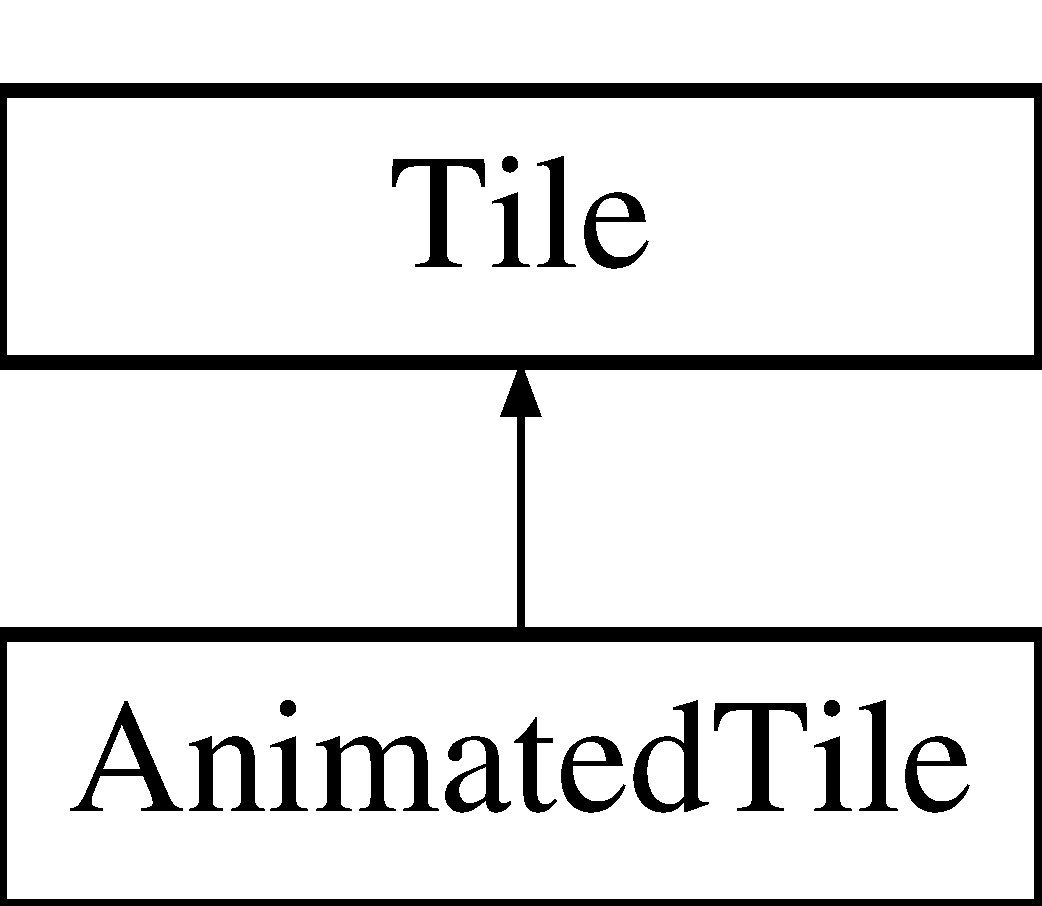
\includegraphics[height=2.000000cm]{struct_animated_tile}
\end{center}
\end{figure}
\subsection*{Metody publiczne}
\begin{DoxyCompactItemize}
\item 
\hypertarget{struct_animated_tile_aceb3d448b5632bb74db019e597beedbb}{{\bfseries Animated\-Tile} (unsigned int \-\_\-x, unsigned int \-\_\-y, double \-\_\-speed, \hyperlink{class_animation}{Animation} \-\_\-an, unsigned int t\-\_\-w, unsigned int t\-\_\-h)}\label{struct_animated_tile_aceb3d448b5632bb74db019e597beedbb}

\end{DoxyCompactItemize}
\subsection*{Atrybuty publiczne}
\begin{DoxyCompactItemize}
\item 
\hypertarget{struct_animated_tile_aed6104567115812838040572ff02a3e5}{unsigned int {\bfseries steps}}\label{struct_animated_tile_aed6104567115812838040572ff02a3e5}

\item 
\hypertarget{struct_animated_tile_a85867438fe971f601b34b85544d8a910}{sf\-::\-Time {\bfseries speed}}\label{struct_animated_tile_a85867438fe971f601b34b85544d8a910}

\item 
\hypertarget{struct_animated_tile_a132b1e4eb01d67e5fb7b78cfb7854266}{\hyperlink{class_animation}{Animation} {\bfseries anim}}\label{struct_animated_tile_a132b1e4eb01d67e5fb7b78cfb7854266}

\item 
\hypertarget{struct_animated_tile_a604a41330b7494c623bb2738baa1fb25}{\hyperlink{class_animated_tex}{Animated\-Tex} {\bfseries txt}}\label{struct_animated_tile_a604a41330b7494c623bb2738baa1fb25}

\end{DoxyCompactItemize}


\subsection{Opis szczegółowy}
struktura animowanego kafla 

rozszerza kafel o możliwość animacji 

Dokumentacja dla tej struktury została wygenerowana z pliku\-:\begin{DoxyCompactItemize}
\item 
Map\-System/Tiles.\-h\end{DoxyCompactItemize}

\hypertarget{class_animation}{\section{Dokumentacja klasy Animation}
\label{class_animation}\index{Animation@{Animation}}
}


Klasa przechowująca klatki animacji i ich teksture.  




{\ttfamily \#include $<$Animation.\-hpp$>$}

\subsection*{Metody publiczne}
\begin{DoxyCompactItemize}
\item 
\hypertarget{class_animation_ada4bef5d91687cdd610a830bd90093f9}{void \hyperlink{class_animation_ada4bef5d91687cdd610a830bd90093f9}{set\-Tile\-Size} (unsigned int width, unsigned int height)}\label{class_animation_ada4bef5d91687cdd610a830bd90093f9}

\begin{DoxyCompactList}\small\item\em ustawia wiekość kafla \end{DoxyCompactList}\item 
void \hyperlink{class_animation_a486ee5fa2d40ae90f227a19866998c91}{add\-Frame} (sf\-::\-Int\-Rect rect)
\begin{DoxyCompactList}\small\item\em dodaje klatke animacji \end{DoxyCompactList}\item 
void \hyperlink{class_animation_ad55efa0c04a03239a8c176f1710b7a9b}{add\-Frame\-G\-I\-D} (unsigned int i)
\begin{DoxyCompactList}\small\item\em dodaje klatke \end{DoxyCompactList}\item 
void \hyperlink{class_animation_a8528dea500d55c9849ab6d3c30ae15eb}{set\-Tileset} (const sf\-::\-Texture \&texture)
\begin{DoxyCompactList}\small\item\em ustawia tileset z animacjami \end{DoxyCompactList}\item 
const sf\-::\-Texture $\ast$ \hyperlink{class_animation_aafed5696c35b893bb721aa1303d5e84f}{get\-Sprite\-Sheet} () const 
\begin{DoxyCompactList}\small\item\em zwraca tileset \end{DoxyCompactList}\item 
std\-::size\-\_\-t \hyperlink{class_animation_aa8dc627c1800fcad9b9e53c9a102ded3}{get\-Size} () const 
\begin{DoxyCompactList}\small\item\em zwraca ilość klatek w animacji \end{DoxyCompactList}\item 
const sf\-::\-Int\-Rect \& \hyperlink{class_animation_ad587678b331518e926b19b807b153daa}{get\-Frame} (std\-::size\-\_\-t n) const 
\begin{DoxyCompactList}\small\item\em zwraca klatke \end{DoxyCompactList}\end{DoxyCompactItemize}


\subsection{Opis szczegółowy}
Klasa przechowująca klatki animacji i ich teksture. 

\subsection{Dokumentacja funkcji składowych}
\hypertarget{class_animation_a486ee5fa2d40ae90f227a19866998c91}{\index{Animation@{Animation}!add\-Frame@{add\-Frame}}
\index{add\-Frame@{add\-Frame}!Animation@{Animation}}
\subsubsection[{add\-Frame}]{\setlength{\rightskip}{0pt plus 5cm}void Animation\-::add\-Frame (
\begin{DoxyParamCaption}
\item[{sf\-::\-Int\-Rect}]{rect}
\end{DoxyParamCaption}
)}}\label{class_animation_a486ee5fa2d40ae90f227a19866998c91}


dodaje klatke animacji 


\begin{DoxyParams}{Parametry}
{\em rect} & klatka animacji \\
\hline
\end{DoxyParams}
\begin{DoxyReturn}{Zwraca}
null 
\end{DoxyReturn}
\hypertarget{class_animation_ad55efa0c04a03239a8c176f1710b7a9b}{\index{Animation@{Animation}!add\-Frame\-G\-I\-D@{add\-Frame\-G\-I\-D}}
\index{add\-Frame\-G\-I\-D@{add\-Frame\-G\-I\-D}!Animation@{Animation}}
\subsubsection[{add\-Frame\-G\-I\-D}]{\setlength{\rightskip}{0pt plus 5cm}void Animation\-::add\-Frame\-G\-I\-D (
\begin{DoxyParamCaption}
\item[{unsigned int}]{G\-I\-D}
\end{DoxyParamCaption}
)}}\label{class_animation_ad55efa0c04a03239a8c176f1710b7a9b}


dodaje klatke 

dodaje klatke na podstawie G\-I\-D(przeliczonych współrzędnych na wielkość w kaflach) a nie współrzędnych całej tekstury 
\begin{DoxyParams}{Parametry}
{\em G\-I\-D} & gid klatki \\
\hline
\end{DoxyParams}
\begin{DoxyReturn}{Zwraca}
null 
\end{DoxyReturn}
\hypertarget{class_animation_ad587678b331518e926b19b807b153daa}{\index{Animation@{Animation}!get\-Frame@{get\-Frame}}
\index{get\-Frame@{get\-Frame}!Animation@{Animation}}
\subsubsection[{get\-Frame}]{\setlength{\rightskip}{0pt plus 5cm}const sf\-::\-Int\-Rect \& Animation\-::get\-Frame (
\begin{DoxyParamCaption}
\item[{std\-::size\-\_\-t}]{n}
\end{DoxyParamCaption}
) const}}\label{class_animation_ad587678b331518e926b19b807b153daa}


zwraca klatke 

zwraca klatke z vectora klatek 
\begin{DoxyParams}{Parametry}
{\em numer} & klatki \\
\hline
\end{DoxyParams}
\begin{DoxyReturn}{Zwraca}
referencja do klatki animacji 
\end{DoxyReturn}
\hypertarget{class_animation_aa8dc627c1800fcad9b9e53c9a102ded3}{\index{Animation@{Animation}!get\-Size@{get\-Size}}
\index{get\-Size@{get\-Size}!Animation@{Animation}}
\subsubsection[{get\-Size}]{\setlength{\rightskip}{0pt plus 5cm}std\-::size\-\_\-t Animation\-::get\-Size (
\begin{DoxyParamCaption}
{}
\end{DoxyParamCaption}
) const}}\label{class_animation_aa8dc627c1800fcad9b9e53c9a102ded3}


zwraca ilość klatek w animacji 

\begin{DoxyReturn}{Zwraca}
ilość klatek 
\end{DoxyReturn}
\hypertarget{class_animation_aafed5696c35b893bb721aa1303d5e84f}{\index{Animation@{Animation}!get\-Sprite\-Sheet@{get\-Sprite\-Sheet}}
\index{get\-Sprite\-Sheet@{get\-Sprite\-Sheet}!Animation@{Animation}}
\subsubsection[{get\-Sprite\-Sheet}]{\setlength{\rightskip}{0pt plus 5cm}const sf\-::\-Texture $\ast$ Animation\-::get\-Sprite\-Sheet (
\begin{DoxyParamCaption}
{}
\end{DoxyParamCaption}
) const}}\label{class_animation_aafed5696c35b893bb721aa1303d5e84f}


zwraca tileset 

\begin{DoxyReturn}{Zwraca}
wskaźnik do tileseta 
\end{DoxyReturn}
\hypertarget{class_animation_a8528dea500d55c9849ab6d3c30ae15eb}{\index{Animation@{Animation}!set\-Tileset@{set\-Tileset}}
\index{set\-Tileset@{set\-Tileset}!Animation@{Animation}}
\subsubsection[{set\-Tileset}]{\setlength{\rightskip}{0pt plus 5cm}void Animation\-::set\-Tileset (
\begin{DoxyParamCaption}
\item[{const sf\-::\-Texture \&}]{texture}
\end{DoxyParamCaption}
)}}\label{class_animation_a8528dea500d55c9849ab6d3c30ae15eb}


ustawia tileset z animacjami 


\begin{DoxyParams}{Parametry}
{\em texture} & tileset \\
\hline
\end{DoxyParams}


Dokumentacja dla tej klasy została wygenerowana z plików\-:\begin{DoxyCompactItemize}
\item 
Animated\-Sprite/Animation.\-hpp\item 
Animated\-Sprite/Animation.\-cpp\end{DoxyCompactItemize}

\hypertarget{struct_background_tile}{\section{Dokumentacja struktury Background\-Tile}
\label{struct_background_tile}\index{Background\-Tile@{Background\-Tile}}
}


struktura dekoracyjnego kafla  




{\ttfamily \#include $<$Tiles.\-h$>$}

Diagram dziedziczenia dla Background\-Tile\begin{figure}[H]
\begin{center}
\leavevmode
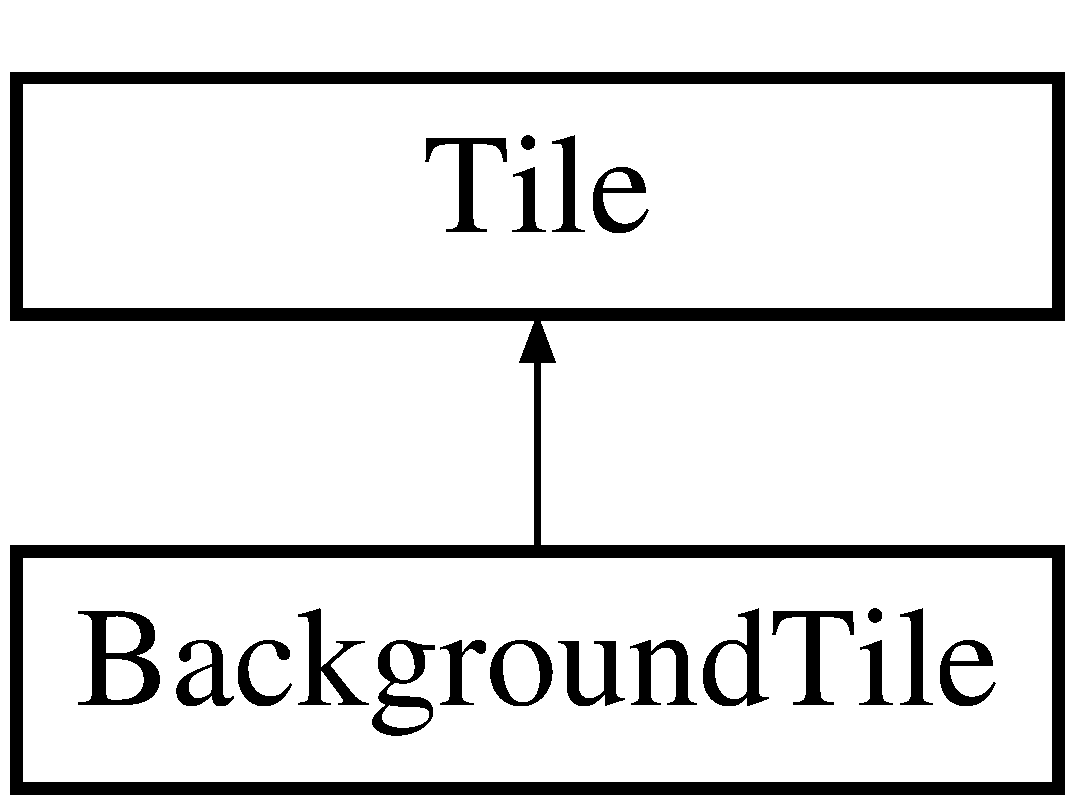
\includegraphics[height=2.000000cm]{struct_background_tile}
\end{center}
\end{figure}
\subsection*{Metody publiczne}
\begin{DoxyCompactItemize}
\item 
\hypertarget{struct_background_tile_ae57f73e5ceef82262afd018d13ede543}{{\bfseries Background\-Tile} (const sf\-::\-Uint32 \-\_\-x, const sf\-::\-Uint32 \-\_\-y, const sf\-::\-Uint32 \-\_\-gid)}\label{struct_background_tile_ae57f73e5ceef82262afd018d13ede543}

\end{DoxyCompactItemize}
\subsection*{Dodatkowe Dziedziczone Składowe}


\subsection{Opis szczegółowy}
struktura dekoracyjnego kafla 

Dokumentacja dla tej struktury została wygenerowana z pliku\-:\begin{DoxyCompactItemize}
\item 
Map\-System/Tiles.\-h\end{DoxyCompactItemize}

\hypertarget{class_button}{\section{Dokumentacja klasy Button}
\label{class_button}\index{Button@{Button}}
}
\subsection*{Metody publiczne}
\begin{DoxyCompactItemize}
\item 
\hypertarget{class_button_af60c30b0db01c76e6940c617364fbb45}{{\bfseries Button} (sf\-::\-Text new\-\_\-text, sf\-::\-Texture \&txt, sf\-::\-Vector2f postion)}\label{class_button_af60c30b0db01c76e6940c617364fbb45}

\item 
\hypertarget{class_button_adf65892636ea303a84e1391106ea7cb0}{void {\bfseries draw} (sf\-::\-Render\-Window \&window)}\label{class_button_adf65892636ea303a84e1391106ea7cb0}

\item 
\hypertarget{class_button_ac66ca457d1227688d738479ff633caab}{bool {\bfseries click} (sf\-::\-Render\-Window \&window, sf\-::\-Sprite sprite, sf\-::\-Event \&event)}\label{class_button_ac66ca457d1227688d738479ff633caab}

\item 
\hypertarget{class_button_a9d9b8af0b3053dd07eef9c3832e5a23c}{sf\-::\-Sprite {\bfseries get\-Sprite} ()}\label{class_button_a9d9b8af0b3053dd07eef9c3832e5a23c}

\end{DoxyCompactItemize}
\subsection*{Statyczne metody publiczne}
\begin{DoxyCompactItemize}
\item 
\hypertarget{class_button_aaeb6570a11ed86b505a31cc250a7c7fb}{static \hyperlink{class_button}{Button} {\bfseries create} (sf\-::\-Text new\-\_\-text, sf\-::\-Texture \&txt, sf\-::\-Vector2f postion)}\label{class_button_aaeb6570a11ed86b505a31cc250a7c7fb}

\end{DoxyCompactItemize}


Dokumentacja dla tej klasy została wygenerowana z plików\-:\begin{DoxyCompactItemize}
\item 
Dialog\-System/Button.\-h\item 
Dialog\-System/Button.\-cpp\end{DoxyCompactItemize}

\hypertarget{class_dialog}{\section{Dokumentacja klasy Dialog}
\label{class_dialog}\index{Dialog@{Dialog}}
}
\subsection*{Metody publiczne}
\begin{DoxyCompactItemize}
\item 
\hypertarget{class_dialog_a09bd324cf3edb083b78f8c5924a7da57}{{\bfseries Dialog} (sf\-::\-Color bgcolor)}\label{class_dialog_a09bd324cf3edb083b78f8c5924a7da57}

\item 
\hypertarget{class_dialog_accb9135a31533d3a7ce9f4555e5035a2}{void {\bfseries show} (sf\-::\-Render\-Window \&window, sf\-::\-Text \&text, sf\-::\-Vector2f \-\_\-size, sf\-::\-Vector2f position)}\label{class_dialog_accb9135a31533d3a7ce9f4555e5035a2}

\end{DoxyCompactItemize}


Dokumentacja dla tej klasy została wygenerowana z plików\-:\begin{DoxyCompactItemize}
\item 
Dialog\-System/Dialog.\-h\item 
Dialog\-System/Dialog.\-cpp\end{DoxyCompactItemize}

\hypertarget{class_entity}{\section{Dokumentacja klasy Entity}
\label{class_entity}\index{Entity@{Entity}}
}


Klasa bytu, który może poruszać sie po mapie, i mieć animacje.  




{\ttfamily \#include $<$Entity.\-hpp$>$}

Diagram dziedziczenia dla Entity\begin{figure}[H]
\begin{center}
\leavevmode
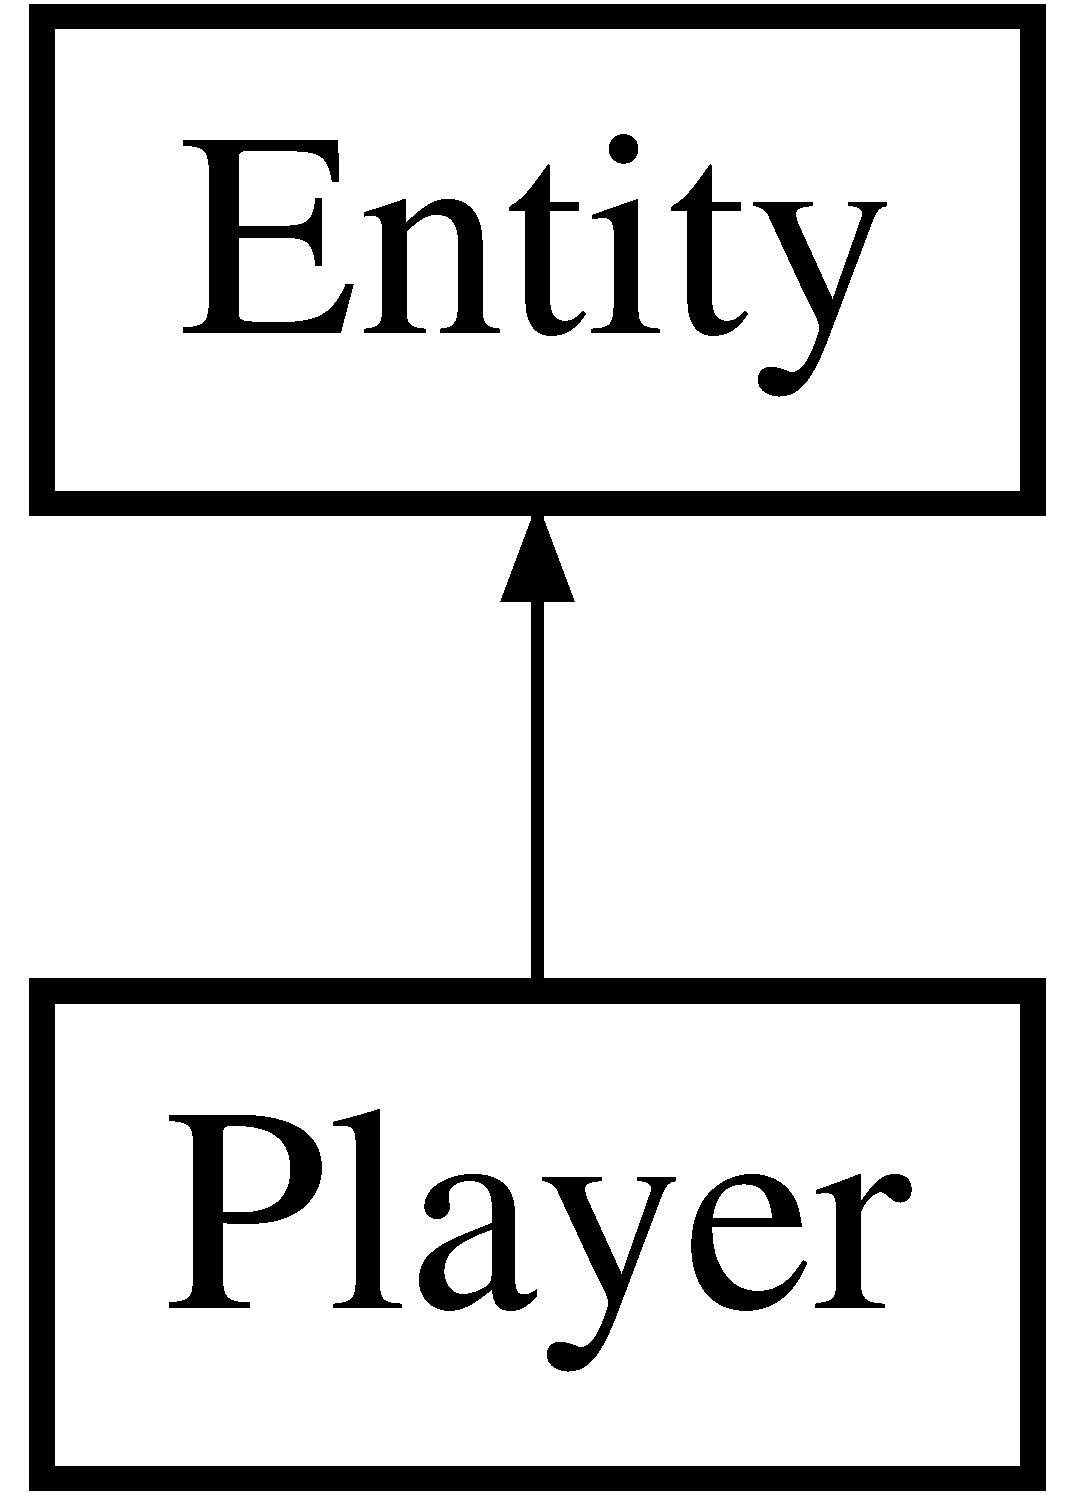
\includegraphics[height=2.000000cm]{class_entity}
\end{center}
\end{figure}
\subsection*{Metody publiczne}
\begin{DoxyCompactItemize}
\item 
\hyperlink{class_entity_a8e13fe1a39745c6912d62e252edc0709}{Entity} (unsigned int x=32, unsigned int y=32)
\begin{DoxyCompactList}\small\item\em Konstruktor. \end{DoxyCompactList}\item 
bool \hyperlink{class_entity_a2d6182aff5fb37582bdb52abfd1d7fde}{load} (const std\-::string path)
\begin{DoxyCompactList}\small\item\em Ładuje animacje z pliku. \end{DoxyCompactList}\item 
\hypertarget{class_entity_a10f39c35a26c9a808676c70eb2742c7b}{void \hyperlink{class_entity_a10f39c35a26c9a808676c70eb2742c7b}{move\-Down} ()}\label{class_entity_a10f39c35a26c9a808676c70eb2742c7b}

\begin{DoxyCompactList}\small\item\em Porusza obiekt w dół i animuje ruch. \end{DoxyCompactList}\item 
\hypertarget{class_entity_a7775cd62029bcba5875a6d9e28172d0e}{void \hyperlink{class_entity_a7775cd62029bcba5875a6d9e28172d0e}{move\-Left} ()}\label{class_entity_a7775cd62029bcba5875a6d9e28172d0e}

\begin{DoxyCompactList}\small\item\em Porusza obiekt w lewo i animuje ruch. \end{DoxyCompactList}\item 
\hypertarget{class_entity_a72d22f873f82e23e424f58d42a45162c}{void \hyperlink{class_entity_a72d22f873f82e23e424f58d42a45162c}{move\-Right} ()}\label{class_entity_a72d22f873f82e23e424f58d42a45162c}

\begin{DoxyCompactList}\small\item\em Porusza obiekt w prawo i animuje ruch. \end{DoxyCompactList}\item 
\hypertarget{class_entity_ab72296eceda3417186ccdb2b2dd64ff8}{void \hyperlink{class_entity_ab72296eceda3417186ccdb2b2dd64ff8}{move\-Up} ()}\label{class_entity_ab72296eceda3417186ccdb2b2dd64ff8}

\begin{DoxyCompactList}\small\item\em Porusza obiekt w góre i animuje ruch. \end{DoxyCompactList}\item 
\hypertarget{class_entity_a00b6eeaf99b35c8f8b10b5fbfc1baf4f}{void \hyperlink{class_entity_a00b6eeaf99b35c8f8b10b5fbfc1baf4f}{update} ()}\label{class_entity_a00b6eeaf99b35c8f8b10b5fbfc1baf4f}

\begin{DoxyCompactList}\small\item\em Odświeża animacje. \end{DoxyCompactList}\item 
\hypertarget{class_entity_a651d16aa7cc3046e9387912496685ead}{void \hyperlink{class_entity_a651d16aa7cc3046e9387912496685ead}{idle} ()}\label{class_entity_a651d16aa7cc3046e9387912496685ead}

\begin{DoxyCompactList}\small\item\em idle \end{DoxyCompactList}\item 
void \hyperlink{class_entity_af6eeb3e2ab8bfe2885bab25f156ed78b}{set\-Position} (unsigned int, unsigned int)
\begin{DoxyCompactList}\small\item\em Ustawia pozycje ( w kaflach ) \end{DoxyCompactList}\item 
void \hyperlink{class_entity_a727a12d714ee329c92b62f3ba60f79f9}{set\-Position\-Float} (float, float)
\begin{DoxyCompactList}\small\item\em Ustawia pozycje ( float ) \end{DoxyCompactList}\item 
sf\-::\-Vector2u \hyperlink{class_entity_a60954d1d71c33104bf549f39c61dbb9f}{get\-Position} ()
\begin{DoxyCompactList}\small\item\em Zwraca pozycje przeliczoną na kafle. \end{DoxyCompactList}\item 
\hypertarget{class_entity_aa254c3e47aa6d3c4b9e2bbbcc786d93f}{sf\-::\-Vector2f \hyperlink{class_entity_aa254c3e47aa6d3c4b9e2bbbcc786d93f}{get\-Position\-Float} ()}\label{class_entity_aa254c3e47aa6d3c4b9e2bbbcc786d93f}

\begin{DoxyCompactList}\small\item\em Zwraca pozycje w floatcie. \end{DoxyCompactList}\item 
\hypertarget{class_entity_a8a29089df65336842035e9a6b73677f6}{virtual void \hyperlink{class_entity_a8a29089df65336842035e9a6b73677f6}{draw} (sf\-::\-Render\-Target \&target, sf\-::\-Render\-States states) const }\label{class_entity_a8a29089df65336842035e9a6b73677f6}

\begin{DoxyCompactList}\small\item\em Rysuje. \end{DoxyCompactList}\end{DoxyCompactItemize}
\subsection*{Atrybuty chronione}
\begin{DoxyCompactItemize}
\item 
\hypertarget{class_entity_ae9986b41f6b347a36c9692c30e6cb5e7}{unsigned int {\bfseries tile\-\_\-width} = 32}\label{class_entity_ae9986b41f6b347a36c9692c30e6cb5e7}

\item 
\hypertarget{class_entity_aa6c74732076834899b7e3a05744a2109}{unsigned int {\bfseries tile\-\_\-height} = 32}\label{class_entity_aa6c74732076834899b7e3a05744a2109}

\item 
std\-::vector$<$ \hyperlink{class_animation}{Animation} $>$ \hyperlink{class_entity_adca44d97840ac7cff2d91d4d518edbcf}{anims}
\begin{DoxyCompactList}\small\item\em Animacje. \end{DoxyCompactList}\item 
\hyperlink{class_animation}{Animation} $\ast$ \hyperlink{class_entity_a60767e4984ab5817623a970f40c51591}{c\-\_\-anim}
\begin{DoxyCompactList}\small\item\em Aktualna animacja. \end{DoxyCompactList}\item 
\hyperlink{class_animated_tex}{Animated\-Tex} \hyperlink{class_entity_ad968b2c732af4a7087842f31202438fc}{anitex}
\begin{DoxyCompactList}\small\item\em Util. \end{DoxyCompactList}\item 
sf\-::\-Vector2f \hyperlink{class_entity_afc349ec89c2bffef70bf6a1d95603154}{position}
\begin{DoxyCompactList}\small\item\em Pozycja. \end{DoxyCompactList}\item 
sf\-::\-Texture \hyperlink{class_entity_a50a3dffcf26eb1950587414663951267}{tiles}
\begin{DoxyCompactList}\small\item\em Tekstura. \end{DoxyCompactList}\item 
float \hyperlink{class_entity_a1de3d8d9ab8088f61e6726069b26fa60}{speed}
\begin{DoxyCompactList}\small\item\em Szybkość przemieszczania się \end{DoxyCompactList}\item 
sf\-::\-Clock \hyperlink{class_entity_a371e5de242da644dca5e90674eb0c1bc}{\-\_\-clock}
\begin{DoxyCompactList}\small\item\em Zegarek. \end{DoxyCompactList}\item 
bool \hyperlink{class_entity_a819f25d4808e9e06d2e3af164b901350}{nokeypressed}
\begin{DoxyCompactList}\small\item\em klawisz \end{DoxyCompactList}\end{DoxyCompactItemize}


\subsection{Opis szczegółowy}
Klasa bytu, który może poruszać sie po mapie, i mieć animacje. 

\subsection{Dokumentacja konstruktora i destruktora}
\hypertarget{class_entity_a8e13fe1a39745c6912d62e252edc0709}{\index{Entity@{Entity}!Entity@{Entity}}
\index{Entity@{Entity}!Entity@{Entity}}
\subsubsection[{Entity}]{\setlength{\rightskip}{0pt plus 5cm}Entity\-::\-Entity (
\begin{DoxyParamCaption}
\item[{unsigned int}]{x = {\ttfamily 32}, }
\item[{unsigned int}]{y = {\ttfamily 32}}
\end{DoxyParamCaption}
)}}\label{class_entity_a8e13fe1a39745c6912d62e252edc0709}


Konstruktor. 


\begin{DoxyParams}{Parametry}
{\em x,y} & współrzędne \\
\hline
\end{DoxyParams}


\subsection{Dokumentacja funkcji składowych}
\hypertarget{class_entity_a60954d1d71c33104bf549f39c61dbb9f}{\index{Entity@{Entity}!get\-Position@{get\-Position}}
\index{get\-Position@{get\-Position}!Entity@{Entity}}
\subsubsection[{get\-Position}]{\setlength{\rightskip}{0pt plus 5cm}sf\-::\-Vector2u Entity\-::get\-Position (
\begin{DoxyParamCaption}
{}
\end{DoxyParamCaption}
)}}\label{class_entity_a60954d1d71c33104bf549f39c61dbb9f}


Zwraca pozycje przeliczoną na kafle. 

\begin{DoxyReturn}{Zwraca}
Pozycja 
\end{DoxyReturn}
\hypertarget{class_entity_a2d6182aff5fb37582bdb52abfd1d7fde}{\index{Entity@{Entity}!load@{load}}
\index{load@{load}!Entity@{Entity}}
\subsubsection[{load}]{\setlength{\rightskip}{0pt plus 5cm}bool Entity\-::load (
\begin{DoxyParamCaption}
\item[{const std\-::string}]{path}
\end{DoxyParamCaption}
)}}\label{class_entity_a2d6182aff5fb37582bdb52abfd1d7fde}


Ładuje animacje z pliku. 

Możliwe dwa formaty plików, informacje logowane do pliku. 
\begin{DoxyParams}{Parametry}
{\em path} & -\/ ścieżka do pliku X\-M\-L \\
\hline
\end{DoxyParams}
\begin{DoxyReturn}{Zwraca}
Powodzenie operacji 
\end{DoxyReturn}
\hypertarget{class_entity_af6eeb3e2ab8bfe2885bab25f156ed78b}{\index{Entity@{Entity}!set\-Position@{set\-Position}}
\index{set\-Position@{set\-Position}!Entity@{Entity}}
\subsubsection[{set\-Position}]{\setlength{\rightskip}{0pt plus 5cm}void Entity\-::set\-Position (
\begin{DoxyParamCaption}
\item[{unsigned int}]{x, }
\item[{unsigned int}]{y}
\end{DoxyParamCaption}
)}}\label{class_entity_af6eeb3e2ab8bfe2885bab25f156ed78b}


Ustawia pozycje ( w kaflach ) 


\begin{DoxyParams}{Parametry}
{\em xy} & -\/ współrzędne \\
\hline
\end{DoxyParams}
\hypertarget{class_entity_a727a12d714ee329c92b62f3ba60f79f9}{\index{Entity@{Entity}!set\-Position\-Float@{set\-Position\-Float}}
\index{set\-Position\-Float@{set\-Position\-Float}!Entity@{Entity}}
\subsubsection[{set\-Position\-Float}]{\setlength{\rightskip}{0pt plus 5cm}void Entity\-::set\-Position\-Float (
\begin{DoxyParamCaption}
\item[{float}]{x, }
\item[{float}]{y}
\end{DoxyParamCaption}
)}}\label{class_entity_a727a12d714ee329c92b62f3ba60f79f9}


Ustawia pozycje ( float ) 


\begin{DoxyParams}{Parametry}
{\em xy} & -\/ współrzędne \\
\hline
\end{DoxyParams}


\subsection{Dokumentacja atrybutów składowych}
\hypertarget{class_entity_a371e5de242da644dca5e90674eb0c1bc}{\index{Entity@{Entity}!\-\_\-clock@{\-\_\-clock}}
\index{\-\_\-clock@{\-\_\-clock}!Entity@{Entity}}
\subsubsection[{\-\_\-clock}]{\setlength{\rightskip}{0pt plus 5cm}sf\-::\-Clock Entity\-::\-\_\-clock\hspace{0.3cm}{\ttfamily [protected]}}}\label{class_entity_a371e5de242da644dca5e90674eb0c1bc}


Zegarek. 


\begin{DoxyItemize}
\item 
\end{DoxyItemize}\hypertarget{class_entity_adca44d97840ac7cff2d91d4d518edbcf}{\index{Entity@{Entity}!anims@{anims}}
\index{anims@{anims}!Entity@{Entity}}
\subsubsection[{anims}]{\setlength{\rightskip}{0pt plus 5cm}std\-::vector$<${\bf Animation}$>$ Entity\-::anims\hspace{0.3cm}{\ttfamily [protected]}}}\label{class_entity_adca44d97840ac7cff2d91d4d518edbcf}


Animacje. 


\begin{DoxyItemize}
\item 
\end{DoxyItemize}\hypertarget{class_entity_ad968b2c732af4a7087842f31202438fc}{\index{Entity@{Entity}!anitex@{anitex}}
\index{anitex@{anitex}!Entity@{Entity}}
\subsubsection[{anitex}]{\setlength{\rightskip}{0pt plus 5cm}{\bf Animated\-Tex} Entity\-::anitex\hspace{0.3cm}{\ttfamily [protected]}}}\label{class_entity_ad968b2c732af4a7087842f31202438fc}


Util. 


\begin{DoxyItemize}
\item 
\end{DoxyItemize}\hypertarget{class_entity_a60767e4984ab5817623a970f40c51591}{\index{Entity@{Entity}!c\-\_\-anim@{c\-\_\-anim}}
\index{c\-\_\-anim@{c\-\_\-anim}!Entity@{Entity}}
\subsubsection[{c\-\_\-anim}]{\setlength{\rightskip}{0pt plus 5cm}{\bf Animation}$\ast$ Entity\-::c\-\_\-anim\hspace{0.3cm}{\ttfamily [protected]}}}\label{class_entity_a60767e4984ab5817623a970f40c51591}


Aktualna animacja. 


\begin{DoxyItemize}
\item 
\end{DoxyItemize}\hypertarget{class_entity_a819f25d4808e9e06d2e3af164b901350}{\index{Entity@{Entity}!nokeypressed@{nokeypressed}}
\index{nokeypressed@{nokeypressed}!Entity@{Entity}}
\subsubsection[{nokeypressed}]{\setlength{\rightskip}{0pt plus 5cm}bool Entity\-::nokeypressed\hspace{0.3cm}{\ttfamily [protected]}}}\label{class_entity_a819f25d4808e9e06d2e3af164b901350}


klawisz 


\begin{DoxyItemize}
\item 
\end{DoxyItemize}\hypertarget{class_entity_afc349ec89c2bffef70bf6a1d95603154}{\index{Entity@{Entity}!position@{position}}
\index{position@{position}!Entity@{Entity}}
\subsubsection[{position}]{\setlength{\rightskip}{0pt plus 5cm}sf\-::\-Vector2f Entity\-::position\hspace{0.3cm}{\ttfamily [protected]}}}\label{class_entity_afc349ec89c2bffef70bf6a1d95603154}


Pozycja. 


\begin{DoxyItemize}
\item 
\end{DoxyItemize}\hypertarget{class_entity_a1de3d8d9ab8088f61e6726069b26fa60}{\index{Entity@{Entity}!speed@{speed}}
\index{speed@{speed}!Entity@{Entity}}
\subsubsection[{speed}]{\setlength{\rightskip}{0pt plus 5cm}float Entity\-::speed\hspace{0.3cm}{\ttfamily [protected]}}}\label{class_entity_a1de3d8d9ab8088f61e6726069b26fa60}


Szybkość przemieszczania się 


\begin{DoxyItemize}
\item 
\end{DoxyItemize}\hypertarget{class_entity_a50a3dffcf26eb1950587414663951267}{\index{Entity@{Entity}!tiles@{tiles}}
\index{tiles@{tiles}!Entity@{Entity}}
\subsubsection[{tiles}]{\setlength{\rightskip}{0pt plus 5cm}sf\-::\-Texture Entity\-::tiles\hspace{0.3cm}{\ttfamily [protected]}}}\label{class_entity_a50a3dffcf26eb1950587414663951267}


Tekstura. 


\begin{DoxyItemize}
\item 
\end{DoxyItemize}

Dokumentacja dla tej klasy została wygenerowana z plików\-:\begin{DoxyCompactItemize}
\item 
Person/Entity.\-hpp\item 
Person/Entity.\-cpp\end{DoxyCompactItemize}

\hypertarget{class_equipment}{\section{Dokumentacja klasy Equipment}
\label{class_equipment}\index{Equipment@{Equipment}}
}
\subsection*{Metody publiczne}
\begin{DoxyCompactItemize}
\item 
\hypertarget{class_equipment_af18f784a9c9c38469a114748b08b47cb}{{\bfseries Equipment} (sf\-::\-Texture \&txt, sf\-::\-Vector2f position)}\label{class_equipment_af18f784a9c9c38469a114748b08b47cb}

\item 
\hypertarget{class_equipment_a8a6f3280ee540b9b812688a1d6fbbb3d}{void {\bfseries add\-Item} (\hyperlink{class_equipment_item}{Equipment\-Item} new\-\_\-item)}\label{class_equipment_a8a6f3280ee540b9b812688a1d6fbbb3d}

\item 
\hypertarget{class_equipment_ad80e042eb307687437579e8a6a307955}{void {\bfseries remove\-Item} (int id)}\label{class_equipment_ad80e042eb307687437579e8a6a307955}

\item 
\hypertarget{class_equipment_a0c4e6291ad7082d049a6d830df923a80}{void {\bfseries draw} (sf\-::\-Render\-Window \&window)}\label{class_equipment_a0c4e6291ad7082d049a6d830df923a80}

\item 
\hypertarget{class_equipment_aa10e2241bfd394059dd178e414583944}{void {\bfseries load\-Texture} (const std\-::string name)}\label{class_equipment_aa10e2241bfd394059dd178e414583944}

\item 
\hypertarget{class_equipment_a3921fcd8ded253cdcda46ea6b25c5013}{void {\bfseries show\-Box} (sf\-::\-Render\-Window \&window, sf\-::\-Event \&event)}\label{class_equipment_a3921fcd8ded253cdcda46ea6b25c5013}

\end{DoxyCompactItemize}


Dokumentacja dla tej klasy została wygenerowana z plików\-:\begin{DoxyCompactItemize}
\item 
Dialog\-System/Equipment.\-h\item 
Dialog\-System/Equipment.\-cpp\end{DoxyCompactItemize}

\hypertarget{class_equipment_item}{\section{Dokumentacja klasy Equipment\-Item}
\label{class_equipment_item}\index{Equipment\-Item@{Equipment\-Item}}
}
\subsection*{Metody publiczne}
\begin{DoxyCompactItemize}
\item 
\hypertarget{class_equipment_item_a507d9df3d88123f1dec109899763f383}{{\bfseries Equipment\-Item} (sf\-::\-Texture \&txt, std\-::string T\-E\-X\-T, int font\-\_\-size, sf\-::\-Color font\-\_\-color, sf\-::\-Vector2f box\-\_\-size, sf\-::\-Color box\-\_\-color, sf\-::\-Color outline\-\_\-color, float thin\-\_\-outline, sf\-::\-Font \&font, uint8\-\_\-t transparent)}\label{class_equipment_item_a507d9df3d88123f1dec109899763f383}

\item 
\hypertarget{class_equipment_item_a2d3ecb4dbfa1203667f23d20ce0a9079}{void {\bfseries set\-Position} (sf\-::\-Vector2f position, float margin\-\_\-box, float text\-\_\-margin\-\_\-top, float text\-\_\-margin\-\_\-left)}\label{class_equipment_item_a2d3ecb4dbfa1203667f23d20ce0a9079}

\item 
\hypertarget{class_equipment_item_a296ad994b66b1030a785d25db6d6de88}{void {\bfseries show\-Box} (sf\-::\-Render\-Window \&window)}\label{class_equipment_item_a296ad994b66b1030a785d25db6d6de88}

\item 
\hypertarget{class_equipment_item_a672338412d6a25355d207365463fdbfb}{void {\bfseries draw} (sf\-::\-Render\-Window \&window)}\label{class_equipment_item_a672338412d6a25355d207365463fdbfb}

\item 
\hypertarget{class_equipment_item_a272b4fbf364401f4da062989fd378279}{bool {\bfseries click} (sf\-::\-Render\-Window \&window, sf\-::\-Event \&event)}\label{class_equipment_item_a272b4fbf364401f4da062989fd378279}

\item 
\hypertarget{class_equipment_item_a0bfae8fad4d05892cf8409b505421617}{sf\-::\-Sprite {\bfseries get\-Sprite} ()}\label{class_equipment_item_a0bfae8fad4d05892cf8409b505421617}

\end{DoxyCompactItemize}


Dokumentacja dla tej klasy została wygenerowana z plików\-:\begin{DoxyCompactItemize}
\item 
Dialog\-System/Equipment\-Item.\-h\item 
Dialog\-System/Equipment\-Item.\-cpp\end{DoxyCompactItemize}

\hypertarget{struct_item}{\section{Dokumentacja struktury Item}
\label{struct_item}\index{Item@{Item}}
}
\subsection*{Metody publiczne}
\begin{DoxyCompactItemize}
\item 
\hypertarget{struct_item_a19f39018c0a5828820d71010379c3ed2}{{\bfseries Item} (unsigned int \-\_\-x, unsigned int \-\_\-y, unsigned int \-\_\-gid, unsigned int \-\_\-id, bool \-\_\-v)}\label{struct_item_a19f39018c0a5828820d71010379c3ed2}

\item 
\hypertarget{struct_item_aec504a524d83a24df80e6585c7db7792}{{\bfseries Item} (const \hyperlink{struct_item}{Item} \&tmp)}\label{struct_item_aec504a524d83a24df80e6585c7db7792}

\item 
\hypertarget{struct_item_a8e4ebdab0cc6e9e9cd1156f328d81ca8}{\hyperlink{struct_item}{Item} \& {\bfseries operator=} (const \hyperlink{struct_item}{Item} \&rhs)}\label{struct_item_a8e4ebdab0cc6e9e9cd1156f328d81ca8}

\item 
\hypertarget{struct_item_af46dc96b212e1fe2710e04a6c7b262ff}{bool {\bfseries operator==} (const \hyperlink{struct_item}{Item} \&rhs) const }\label{struct_item_af46dc96b212e1fe2710e04a6c7b262ff}

\end{DoxyCompactItemize}
\subsection*{Atrybuty publiczne}
\begin{DoxyCompactItemize}
\item 
\hypertarget{struct_item_a9d5f77ac922932e7743b4dc0d1fbf67f}{unsigned int {\bfseries x}}\label{struct_item_a9d5f77ac922932e7743b4dc0d1fbf67f}

\item 
\hypertarget{struct_item_a758822c85d6baeadd828cbc0b4ef14b8}{unsigned int {\bfseries y}}\label{struct_item_a758822c85d6baeadd828cbc0b4ef14b8}

\item 
\hypertarget{struct_item_a0b31e0d6e016bc211e6a07ccedaf721f}{unsigned int {\bfseries gid}}\label{struct_item_a0b31e0d6e016bc211e6a07ccedaf721f}

\item 
\hypertarget{struct_item_ae901ac3ab2273113f746340a7db4e388}{int {\bfseries id}}\label{struct_item_ae901ac3ab2273113f746340a7db4e388}

\item 
\hypertarget{struct_item_ad391b381597b6df426c21cc5f3a994a8}{bool {\bfseries valid}}\label{struct_item_ad391b381597b6df426c21cc5f3a994a8}

\end{DoxyCompactItemize}


Dokumentacja dla tej struktury została wygenerowana z pliku\-:\begin{DoxyCompactItemize}
\item 
Map\-System/Item.\-h\end{DoxyCompactItemize}

\hypertarget{struct_item_data}{\section{Dokumentacja struktury Item\-Data}
\label{struct_item_data}\index{Item\-Data@{Item\-Data}}
}
\subsection*{Metody publiczne}
\begin{DoxyCompactItemize}
\item 
\hypertarget{struct_item_data_a8ff460ef078580548de4405309678fe9}{{\bfseries Item\-Data} (I\-T\-E\-M\-\_\-\-T\-Y\-P\-E \-\_\-type, std\-::string \-\_\-desc, std\-::string \-\_\-nam, unsigned int \-\_\-att, unsigned int \-\_\-def, unsigned int \-\_\-qua, unsigned int \-\_\-pri, unsigned int \-\_\-pow, unsigned int \-\_\-spe, unsigned int \-\_\-gid)}\label{struct_item_data_a8ff460ef078580548de4405309678fe9}

\item 
\hypertarget{struct_item_data_a8d02934a6e2a1399eb80b6ee930b69d3}{{\bfseries Item\-Data} (const \hyperlink{struct_item_data}{Item\-Data} \&rhs)}\label{struct_item_data_a8d02934a6e2a1399eb80b6ee930b69d3}

\item 
\hypertarget{struct_item_data_a225fa8658908c97592b5fed58e361228}{\hyperlink{struct_item_data}{Item\-Data} \& {\bfseries operator=} (const \hyperlink{struct_item_data}{Item\-Data} \&rhs)}\label{struct_item_data_a225fa8658908c97592b5fed58e361228}

\item 
\hypertarget{struct_item_data_a2395fbbbfcf43da6092eebdf17aa23df}{bool {\bfseries operator==} (const \hyperlink{struct_item_data}{Item\-Data} \&rhs) const }\label{struct_item_data_a2395fbbbfcf43da6092eebdf17aa23df}

\end{DoxyCompactItemize}
\subsection*{Atrybuty publiczne}
\begin{DoxyCompactItemize}
\item 
\hypertarget{struct_item_data_a5c5156ae0135589ea4b55c6dd98db949}{I\-T\-E\-M\-\_\-\-T\-Y\-P\-E {\bfseries type}}\label{struct_item_data_a5c5156ae0135589ea4b55c6dd98db949}

\item 
\hypertarget{struct_item_data_a8122ea77a63a91c64c28a0f7c4ecc539}{std\-::string {\bfseries description}}\label{struct_item_data_a8122ea77a63a91c64c28a0f7c4ecc539}

\item 
\hypertarget{struct_item_data_afb2976e864aa2c9192ef37655210779e}{std\-::string {\bfseries name}}\label{struct_item_data_afb2976e864aa2c9192ef37655210779e}

\item 
\hypertarget{struct_item_data_aac974de802eb3281a00d20b4f4b00919}{unsigned int {\bfseries attack}}\label{struct_item_data_aac974de802eb3281a00d20b4f4b00919}

\item 
\hypertarget{struct_item_data_a06d5face6e73693026ebc173c2e3cb00}{unsigned int {\bfseries defence}}\label{struct_item_data_a06d5face6e73693026ebc173c2e3cb00}

\item 
\hypertarget{struct_item_data_a794a313d4a37e04c2d56033a0a77e84b}{unsigned int {\bfseries quality}}\label{struct_item_data_a794a313d4a37e04c2d56033a0a77e84b}

\item 
\hypertarget{struct_item_data_a29ee94503d48e86a837070b8bf3a408f}{unsigned int {\bfseries price}}\label{struct_item_data_a29ee94503d48e86a837070b8bf3a408f}

\item 
\hypertarget{struct_item_data_add0c206f5054df876030bc6cbd655911}{unsigned int {\bfseries power}}\label{struct_item_data_add0c206f5054df876030bc6cbd655911}

\item 
\hypertarget{struct_item_data_a58d2216af72e9e608ce69dd620037d86}{double {\bfseries speed}}\label{struct_item_data_a58d2216af72e9e608ce69dd620037d86}

\item 
\hypertarget{struct_item_data_a0d109a02f6200ca17476e721b07b32a9}{unsigned int {\bfseries gid}}\label{struct_item_data_a0d109a02f6200ca17476e721b07b32a9}

\end{DoxyCompactItemize}


Dokumentacja dla tej struktury została wygenerowana z pliku\-:\begin{DoxyCompactItemize}
\item 
Map\-System/Item.\-h\end{DoxyCompactItemize}

\hypertarget{class_item_manager}{\section{Dokumentacja klasy Item\-Manager}
\label{class_item_manager}\index{Item\-Manager@{Item\-Manager}}
}


Manager itemów gracza.  




{\ttfamily \#include $<$Item\-Manager.\-hpp$>$}

\subsection*{Metody publiczne}
\begin{DoxyCompactItemize}
\item 
\hypertarget{class_item_manager_a67fde2ac12d912e419ad0d92b4b12398}{void \hyperlink{class_item_manager_a67fde2ac12d912e419ad0d92b4b12398}{print\-Items} ()}\label{class_item_manager_a67fde2ac12d912e419ad0d92b4b12398}

\begin{DoxyCompactList}\small\item\em Tylko do debugowania. \end{DoxyCompactList}\item 
void \hyperlink{class_item_manager_ad62ffaa692d727adf551a0b6235b66b8}{update} (const sf\-::\-Vector2u \&)
\begin{DoxyCompactList}\small\item\em aktualizuje współrzędne itemów \end{DoxyCompactList}\item 
void \hyperlink{class_item_manager_a128c9c267f271881a68bbe49cfbfa2d8}{add\-Item} (const \hyperlink{struct_item}{Item})
\begin{DoxyCompactList}\small\item\em dodaje item do plecaka \end{DoxyCompactList}\item 
void \hyperlink{class_item_manager_a14f1f8717804441005683f3dc37fd10e}{set\-Picked} (size\-\_\-t)
\begin{DoxyCompactList}\small\item\em ustawia flage picked dla danego I\-D \end{DoxyCompactList}\item 
bool \hyperlink{class_item_manager_a57d93634c5347ef69e4cb7888564e852}{load\-Items} (const std\-::string)
\begin{DoxyCompactList}\small\item\em ładuje dane itemów z pliku. \end{DoxyCompactList}\item 
\hypertarget{class_item_manager_abda651aea3b37cb983e158b2b743a4ca}{bool \hyperlink{class_item_manager_abda651aea3b37cb983e158b2b743a4ca}{is\-Picked} (size\-\_\-t) const }\label{class_item_manager_abda651aea3b37cb983e158b2b743a4ca}

\begin{DoxyCompactList}\small\item\em zwraca wartość czy dany item został już podniesiony \end{DoxyCompactList}\item 
bool \hyperlink{class_item_manager_af9d62b0fb7a8a4d44ad5707be5451bfe}{delete\-Item} (const int)
\begin{DoxyCompactList}\small\item\em usuwa item z plecaka \end{DoxyCompactList}\item 
\hyperlink{struct_item}{Item} \hyperlink{class_item_manager_a670709d080a73fdb1872eb3790945325}{get\-Item} (const int id) const 
\begin{DoxyCompactList}\small\item\em wyszukuje item o danym id \end{DoxyCompactList}\item 
\hyperlink{struct_item_data}{Item\-Data} \hyperlink{class_item_manager_a81a09c9a689b40f8fe4d2d422fa5a4da}{get\-Data} (size\-\_\-t) const 
\begin{DoxyCompactList}\small\item\em zwraca strukture \hyperlink{struct_item_data}{Item\-Data} zawierającą dane o przedmiocie \end{DoxyCompactList}\item 
\hypertarget{class_item_manager_aac4440e4b21628d5e993f9f69411e675}{int \hyperlink{class_item_manager_aac4440e4b21628d5e993f9f69411e675}{get\-G\-I\-D} (size\-\_\-t) const }\label{class_item_manager_aac4440e4b21628d5e993f9f69411e675}

\begin{DoxyCompactList}\small\item\em zwraca G\-I\-D itemu na podstawie I\-D \end{DoxyCompactList}\item 
\hypertarget{class_item_manager_ac5660480a58cf8613abb70ce3aefcf30}{size\-\_\-t \hyperlink{class_item_manager_ac5660480a58cf8613abb70ce3aefcf30}{player\-Item\-Count} () const }\label{class_item_manager_ac5660480a58cf8613abb70ce3aefcf30}

\begin{DoxyCompactList}\small\item\em zwraca liczbe itemów w 'plecaku' \end{DoxyCompactList}\end{DoxyCompactItemize}


\subsection{Opis szczegółowy}
Manager itemów gracza. 

\subsection{Dokumentacja funkcji składowych}
\hypertarget{class_item_manager_a128c9c267f271881a68bbe49cfbfa2d8}{\index{Item\-Manager@{Item\-Manager}!add\-Item@{add\-Item}}
\index{add\-Item@{add\-Item}!ItemManager@{Item\-Manager}}
\subsubsection[{add\-Item}]{\setlength{\rightskip}{0pt plus 5cm}void Item\-Manager\-::add\-Item (
\begin{DoxyParamCaption}
\item[{const {\bf Item}}]{itm}
\end{DoxyParamCaption}
)}}\label{class_item_manager_a128c9c267f271881a68bbe49cfbfa2d8}


dodaje item do plecaka 

wyszukuje w itema o danym id w vectorze, i jeśli item o takim id nie istnieje -\/ dodaje go 
\begin{DoxyParams}{Parametry}
{\em itm} & Itemek \\
\hline
\end{DoxyParams}
\hypertarget{class_item_manager_af9d62b0fb7a8a4d44ad5707be5451bfe}{\index{Item\-Manager@{Item\-Manager}!delete\-Item@{delete\-Item}}
\index{delete\-Item@{delete\-Item}!ItemManager@{Item\-Manager}}
\subsubsection[{delete\-Item}]{\setlength{\rightskip}{0pt plus 5cm}bool Item\-Manager\-::delete\-Item (
\begin{DoxyParamCaption}
\item[{const int}]{id}
\end{DoxyParamCaption}
)}}\label{class_item_manager_af9d62b0fb7a8a4d44ad5707be5451bfe}


usuwa item z plecaka 

wyszukuje item o danym id w vectorze, i jeśli istnieje -\/ usuwa go 
\begin{DoxyParams}{Parametry}
{\em id} & id przedmiotu \\
\hline
\end{DoxyParams}
\begin{DoxyReturn}{Zwraca}
jeśli usunięty true, w przeciwnym wypadku false 
\end{DoxyReturn}
\hypertarget{class_item_manager_a81a09c9a689b40f8fe4d2d422fa5a4da}{\index{Item\-Manager@{Item\-Manager}!get\-Data@{get\-Data}}
\index{get\-Data@{get\-Data}!ItemManager@{Item\-Manager}}
\subsubsection[{get\-Data}]{\setlength{\rightskip}{0pt plus 5cm}{\bf Item\-Data} Item\-Manager\-::get\-Data (
\begin{DoxyParamCaption}
\item[{size\-\_\-t}]{gid}
\end{DoxyParamCaption}
) const}}\label{class_item_manager_a81a09c9a689b40f8fe4d2d422fa5a4da}


zwraca strukture \hyperlink{struct_item_data}{Item\-Data} zawierającą dane o przedmiocie 

wyszukuje itema o danym G\-I\-D (do jednej teksturki może być przypisana tylko jedna specyfikacja) 
\begin{DoxyParams}{Parametry}
{\em gid} & gid przedmiotu \\
\hline
\end{DoxyParams}
\begin{DoxyReturn}{Zwraca}
jeśli znaleziono to \hyperlink{struct_item_data}{Item\-Data} z danymi, jeśli nie to \hyperlink{struct_item_data}{Item\-Data} z wyzerowanymi polami i nazwą \char`\"{}undefined\char`\"{} 
\end{DoxyReturn}
\hypertarget{class_item_manager_a670709d080a73fdb1872eb3790945325}{\index{Item\-Manager@{Item\-Manager}!get\-Item@{get\-Item}}
\index{get\-Item@{get\-Item}!ItemManager@{Item\-Manager}}
\subsubsection[{get\-Item}]{\setlength{\rightskip}{0pt plus 5cm}{\bf Item} Item\-Manager\-::get\-Item (
\begin{DoxyParamCaption}
\item[{const int}]{id}
\end{DoxyParamCaption}
) const}}\label{class_item_manager_a670709d080a73fdb1872eb3790945325}


wyszukuje item o danym id 

wyszukuje item o danym id i jeśli istnieje to zwraca go jeśli nie istnieje zwraca domyślny item 
\begin{DoxyParams}{Parametry}
{\em id} & id przedmiotu \\
\hline
\end{DoxyParams}
\begin{DoxyReturn}{Zwraca}
przedmiot 
\end{DoxyReturn}
\hypertarget{class_item_manager_a57d93634c5347ef69e4cb7888564e852}{\index{Item\-Manager@{Item\-Manager}!load\-Items@{load\-Items}}
\index{load\-Items@{load\-Items}!ItemManager@{Item\-Manager}}
\subsubsection[{load\-Items}]{\setlength{\rightskip}{0pt plus 5cm}bool Item\-Manager\-::load\-Items (
\begin{DoxyParamCaption}
\item[{const std\-::string}]{name}
\end{DoxyParamCaption}
)}}\label{class_item_manager_a57d93634c5347ef69e4cb7888564e852}


ładuje dane itemów z pliku. 

ładuje dane itemów z pliku oraz loguje informacje do pliku 
\begin{DoxyParams}{Parametry}
{\em nazwa} & pliku X\-M\-L z danymi itemów \\
\hline
\end{DoxyParams}
\begin{DoxyReturn}{Zwraca}
powodzenie operacji 
\end{DoxyReturn}
\hypertarget{class_item_manager_a14f1f8717804441005683f3dc37fd10e}{\index{Item\-Manager@{Item\-Manager}!set\-Picked@{set\-Picked}}
\index{set\-Picked@{set\-Picked}!ItemManager@{Item\-Manager}}
\subsubsection[{set\-Picked}]{\setlength{\rightskip}{0pt plus 5cm}void Item\-Manager\-::set\-Picked (
\begin{DoxyParamCaption}
\item[{size\-\_\-t}]{id}
\end{DoxyParamCaption}
)}}\label{class_item_manager_a14f1f8717804441005683f3dc37fd10e}


ustawia flage picked dla danego I\-D 

ustawia bool picked w wektorze 'picked' picked domyślnie ma 1000 slotów a pojedyńczy indeks odpowiada danemu id ma to na celu zablokowania istnienia przedmiotu który został wpisany do pliku mapy przy następnych ładowaniach mapy 
\begin{DoxyParams}{Parametry}
{\em id} & id przedmiotu \\
\hline
\end{DoxyParams}
\begin{DoxyReturn}{Zwraca}
null 
\end{DoxyReturn}
\hypertarget{class_item_manager_ad62ffaa692d727adf551a0b6235b66b8}{\index{Item\-Manager@{Item\-Manager}!update@{update}}
\index{update@{update}!ItemManager@{Item\-Manager}}
\subsubsection[{update}]{\setlength{\rightskip}{0pt plus 5cm}void Item\-Manager\-::update (
\begin{DoxyParamCaption}
\item[{const sf\-::\-Vector2u \&}]{vct}
\end{DoxyParamCaption}
)}}\label{class_item_manager_ad62ffaa692d727adf551a0b6235b66b8}


aktualizuje współrzędne itemów 

aktualizuje współrzędne itemów tj. itemy \char`\"{}chodzą\char`\"{} za graczem, są im przypisywane współrzędne gracza 
\begin{DoxyParams}{Parametry}
{\em vct} & współrzędne \\
\hline
\end{DoxyParams}
\begin{DoxyReturn}{Zwraca}
null 
\end{DoxyReturn}


Dokumentacja dla tej klasy została wygenerowana z plików\-:\begin{DoxyCompactItemize}
\item 
Map\-System/Item\-Manager.\-hpp\item 
Map\-System/Item\-Manager.\-cpp\end{DoxyCompactItemize}

\hypertarget{class_menu}{\section{Dokumentacja klasy Menu}
\label{class_menu}\index{Menu@{Menu}}
}
\subsection*{Metody publiczne}
\begin{DoxyCompactItemize}
\item 
\hypertarget{class_menu_ad9c086bd9613bcd23d6dc5ec600a15f5}{{\bfseries Menu} (sf\-::\-Color default\-\_\-, sf\-::\-Color second, int font\-\_\-size)}\label{class_menu_ad9c086bd9613bcd23d6dc5ec600a15f5}

\item 
\hypertarget{class_menu_a1443dcfd1c1c9844c40658d752c1fbab}{void {\bfseries draw} (sf\-::\-Render\-Window \&window)}\label{class_menu_a1443dcfd1c1c9844c40658d752c1fbab}

\item 
\hypertarget{class_menu_a28db106eeb2454f8699b2b076dab9eaf}{void {\bfseries move\-\_\-pointer} (bool up)}\label{class_menu_a28db106eeb2454f8699b2b076dab9eaf}

\end{DoxyCompactItemize}


Dokumentacja dla tej klasy została wygenerowana z plików\-:\begin{DoxyCompactItemize}
\item 
Dialog\-System/Menu.\-h\item 
Dialog\-System/Menu.\-cpp\end{DoxyCompactItemize}

\hypertarget{struct_n_p_c}{\section{Dokumentacja struktury N\-P\-C}
\label{struct_n_p_c}\index{N\-P\-C@{N\-P\-C}}
}
\subsection*{Metody publiczne}
\begin{DoxyCompactItemize}
\item 
\hypertarget{struct_n_p_c_abf814411b67bede6a6cc1c34c9f29321}{{\bfseries N\-P\-C} (std\-::string, unsigned int, unsigned int, sf\-::\-Vector2u, std\-::string)}\label{struct_n_p_c_abf814411b67bede6a6cc1c34c9f29321}

\item 
\hypertarget{struct_n_p_c_ad403b3bd8aa8cc29aa30b941533ea73a}{bool {\bfseries load} ()}\label{struct_n_p_c_ad403b3bd8aa8cc29aa30b941533ea73a}

\item 
\hypertarget{struct_n_p_c_abf814411b67bede6a6cc1c34c9f29321}{{\bfseries N\-P\-C} (std\-::string, unsigned int, unsigned int, sf\-::\-Vector2u, std\-::string)}\label{struct_n_p_c_abf814411b67bede6a6cc1c34c9f29321}

\end{DoxyCompactItemize}
\subsection*{Atrybuty publiczne}
\begin{DoxyCompactItemize}
\item 
\hypertarget{struct_n_p_c_a275f657bea2e125728a9a9613dd6948f}{std\-::string {\bfseries name}}\label{struct_n_p_c_a275f657bea2e125728a9a9613dd6948f}

\item 
\hypertarget{struct_n_p_c_a2f5b3762132d1955a19441044173b643}{std\-::string {\bfseries file}}\label{struct_n_p_c_a2f5b3762132d1955a19441044173b643}

\item 
\hypertarget{struct_n_p_c_a55f8d51a39bf5e719fbcb187b1bb6907}{std\-::vector$<$ std\-::string $>$ {\bfseries talky}}\label{struct_n_p_c_a55f8d51a39bf5e719fbcb187b1bb6907}

\item 
\hypertarget{struct_n_p_c_a8c9d0b0ba615614d325a0eb0247656fe}{sf\-::\-Vector2u {\bfseries m\-\_\-pos}}\label{struct_n_p_c_a8c9d0b0ba615614d325a0eb0247656fe}

\item 
\hypertarget{struct_n_p_c_a407d030745e6fe60b15f8214d99fd11c}{unsigned int {\bfseries id}}\label{struct_n_p_c_a407d030745e6fe60b15f8214d99fd11c}

\item 
\hypertarget{struct_n_p_c_a89d170cdda416f00ed767ac1d0829199}{unsigned int {\bfseries gid}}\label{struct_n_p_c_a89d170cdda416f00ed767ac1d0829199}

\end{DoxyCompactItemize}


Dokumentacja dla tej struktury została wygenerowana z plików\-:\begin{DoxyCompactItemize}
\item 
Npc\-Manager/N\-P\-C.\-hpp\item 
Person/N\-P\-C.\-hpp\item 
Npc\-Manager/N\-P\-C.\-cpp\item 
Person/N\-P\-C.\-cpp\end{DoxyCompactItemize}

\hypertarget{class_npc_manager}{\section{Dokumentacja klasy Npc\-Manager}
\label{class_npc_manager}\index{Npc\-Manager@{Npc\-Manager}}
}
\subsection*{Metody publiczne}
\begin{DoxyCompactItemize}
\item 
\hypertarget{class_npc_manager_ad8b03b02a432e1e6b5a9d30c7fe5012b}{void {\bfseries add\-N\-P\-C} (\hyperlink{struct_n_p_c}{N\-P\-C} npc)}\label{class_npc_manager_ad8b03b02a432e1e6b5a9d30c7fe5012b}

\item 
\hypertarget{class_npc_manager_a96958d77af8589bcec121495b8765e35}{std\-::size\-\_\-t {\bfseries count\-N\-P\-C} ()}\label{class_npc_manager_a96958d77af8589bcec121495b8765e35}

\item 
\hypertarget{class_npc_manager_af8b70fab9fe96eda76ab16e964c19490}{bool {\bfseries near\-N\-P\-C} (sf\-::\-Vector2u v) const }\label{class_npc_manager_af8b70fab9fe96eda76ab16e964c19490}

\item 
\hypertarget{class_npc_manager_a2e4c9ac382614c021c7167c2bf886220}{void {\bfseries clean} ()}\label{class_npc_manager_a2e4c9ac382614c021c7167c2bf886220}

\end{DoxyCompactItemize}


Dokumentacja dla tej klasy została wygenerowana z plików\-:\begin{DoxyCompactItemize}
\item 
Npc\-Manager/Npc\-Manager.\-hpp\item 
Npc\-Manager/Npc\-Manager.\-cpp\end{DoxyCompactItemize}

\hypertarget{class_player}{\section{Dokumentacja klasy Player}
\label{class_player}\index{Player@{Player}}
}
Diagram dziedziczenia dla Player\begin{figure}[H]
\begin{center}
\leavevmode
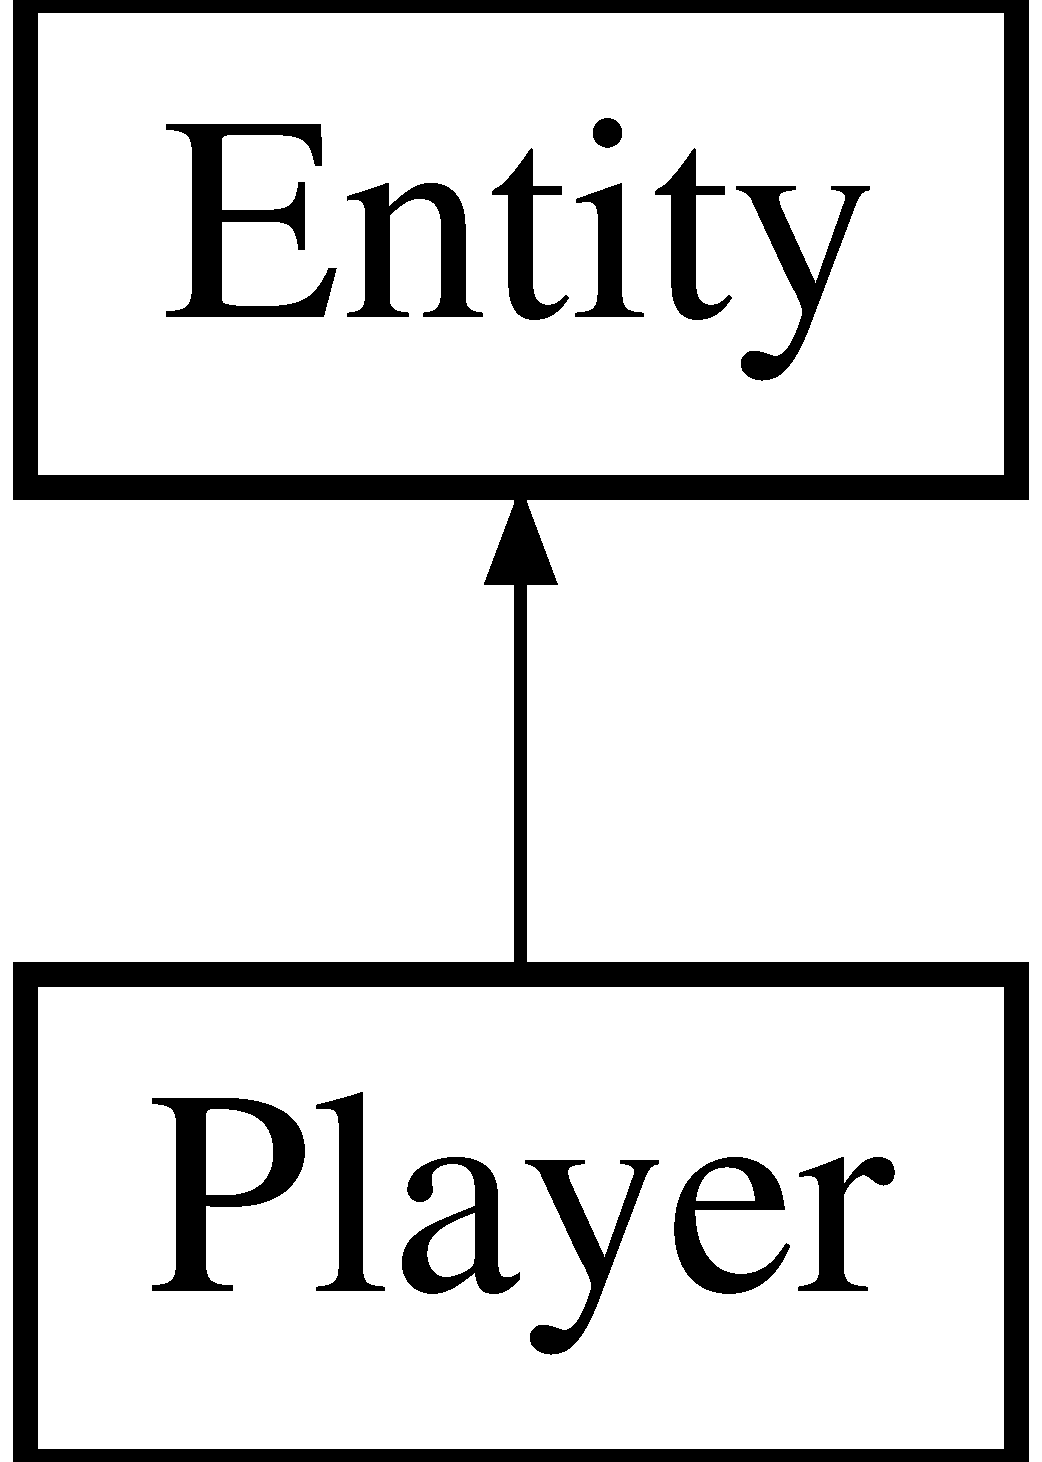
\includegraphics[height=2.000000cm]{class_player}
\end{center}
\end{figure}
\subsection*{Metody publiczne}
\begin{DoxyCompactItemize}
\item 
\hypertarget{class_player_a5baa80c8e1e1cb40e079f28b54b30083}{{\bfseries Player} (unsigned int x=32, unsigned int y=32)}\label{class_player_a5baa80c8e1e1cb40e079f28b54b30083}

\item 
\hypertarget{class_player_a4dd683b1db6aae2f58d23889ff752ad0}{virtual void \hyperlink{class_player_a4dd683b1db6aae2f58d23889ff752ad0}{draw} (sf\-::\-Render\-Target \&target, sf\-::\-Render\-States states) const }\label{class_player_a4dd683b1db6aae2f58d23889ff752ad0}

\begin{DoxyCompactList}\small\item\em Rysuje. \end{DoxyCompactList}\end{DoxyCompactItemize}
\subsection*{Dodatkowe Dziedziczone Składowe}


Dokumentacja dla tej klasy została wygenerowana z plików\-:\begin{DoxyCompactItemize}
\item 
Person/Player.\-hpp\item 
Person/Player.\-cpp\end{DoxyCompactItemize}

\hypertarget{struct_portal_tile}{\section{Dokumentacja struktury Portal\-Tile}
\label{struct_portal_tile}\index{Portal\-Tile@{Portal\-Tile}}
}


struktura portalu  




{\ttfamily \#include $<$Tiles.\-h$>$}

Diagram dziedziczenia dla Portal\-Tile\begin{figure}[H]
\begin{center}
\leavevmode
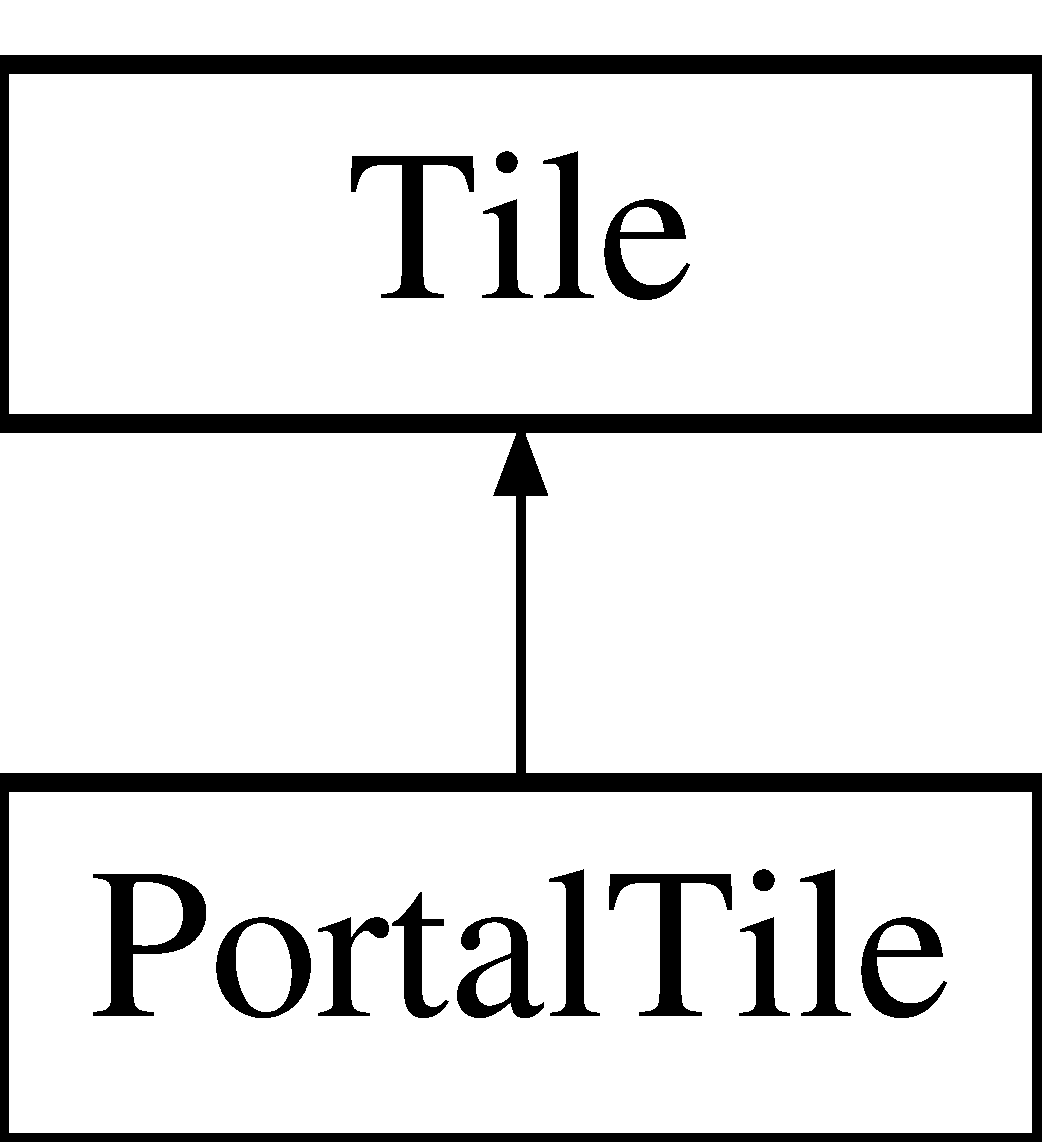
\includegraphics[height=2.000000cm]{struct_portal_tile}
\end{center}
\end{figure}
\subsection*{Metody publiczne}
\begin{DoxyCompactItemize}
\item 
\hypertarget{struct_portal_tile_a9ae99fce73ef382ee6f2e3aa6b3d4388}{{\bfseries Portal\-Tile} (unsigned int \-\_\-x, unsigned int \-\_\-y, unsigned int \-\_\-gid, std\-::string \&\-\_\-file, sf\-::\-Vector2u \-\_\-spawn)}\label{struct_portal_tile_a9ae99fce73ef382ee6f2e3aa6b3d4388}

\end{DoxyCompactItemize}
\subsection*{Atrybuty publiczne}
\begin{DoxyCompactItemize}
\item 
\hypertarget{struct_portal_tile_a0f3d60a453b8b9ec2d9cb14d382451d4}{sf\-::\-Vector2u {\bfseries spawn}}\label{struct_portal_tile_a0f3d60a453b8b9ec2d9cb14d382451d4}

\item 
\hypertarget{struct_portal_tile_aff05b35e46346897a6863877cfeac433}{std\-::string {\bfseries file}}\label{struct_portal_tile_aff05b35e46346897a6863877cfeac433}

\item 
\hypertarget{struct_portal_tile_a1e31f638d7b27e73164b14d3a0650d32}{bool {\bfseries first\-\_\-load}}\label{struct_portal_tile_a1e31f638d7b27e73164b14d3a0650d32}

\end{DoxyCompactItemize}


\subsection{Opis szczegółowy}
struktura portalu 

rozszerza kafel o współrzędne spawnu, nazwe mapy, i informacje o tym czy została załadowana po raz pierwszy 

Dokumentacja dla tej struktury została wygenerowana z pliku\-:\begin{DoxyCompactItemize}
\item 
Map\-System/Tiles.\-h\end{DoxyCompactItemize}

\hypertarget{struct_solid_tile}{\section{Dokumentacja struktury Solid\-Tile}
\label{struct_solid_tile}\index{Solid\-Tile@{Solid\-Tile}}
}


struktura solidnego kafla  




{\ttfamily \#include $<$Tiles.\-h$>$}

Diagram dziedziczenia dla Solid\-Tile\begin{figure}[H]
\begin{center}
\leavevmode
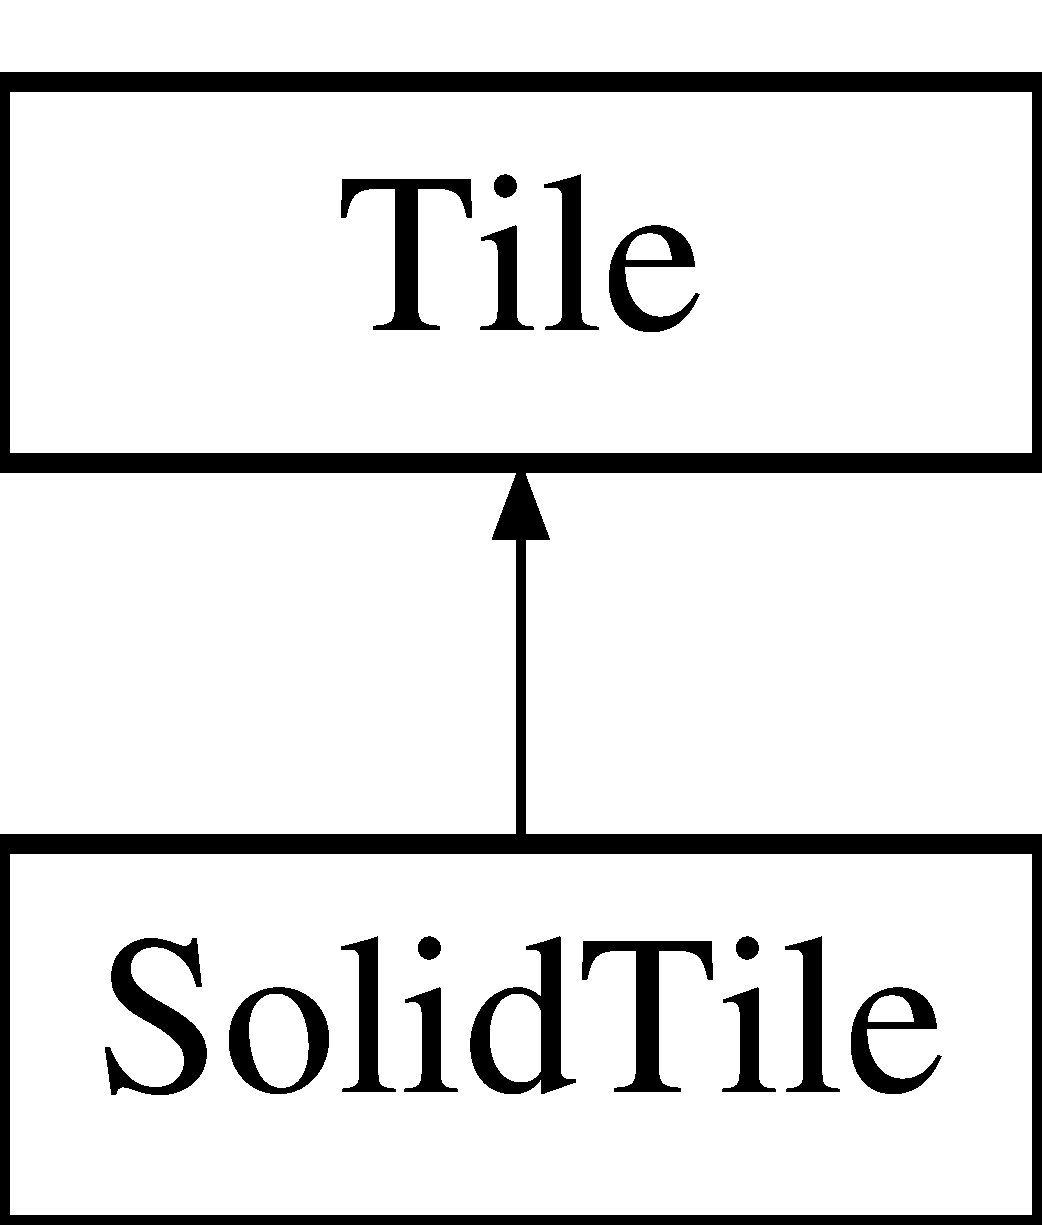
\includegraphics[height=2.000000cm]{struct_solid_tile}
\end{center}
\end{figure}
\subsection*{Metody publiczne}
\begin{DoxyCompactItemize}
\item 
\hypertarget{struct_solid_tile_a64d7a3406a34ddbee80db67e7f0ea508}{{\bfseries Solid\-Tile} (const sf\-::\-Uint32 \-\_\-x, const sf\-::\-Uint32 \-\_\-y, const sf\-::\-Uint32 \-\_\-gid)}\label{struct_solid_tile_a64d7a3406a34ddbee80db67e7f0ea508}

\end{DoxyCompactItemize}
\subsection*{Dodatkowe Dziedziczone Składowe}


\subsection{Opis szczegółowy}
struktura solidnego kafla 

Dokumentacja dla tej struktury została wygenerowana z pliku\-:\begin{DoxyCompactItemize}
\item 
Map\-System/Tiles.\-h\end{DoxyCompactItemize}

\hypertarget{struct_tile}{\section{Dokumentacja struktury Tile}
\label{struct_tile}\index{Tile@{Tile}}
}


struktura bazowa kafla  




{\ttfamily \#include $<$Tiles.\-h$>$}

Diagram dziedziczenia dla Tile\begin{figure}[H]
\begin{center}
\leavevmode
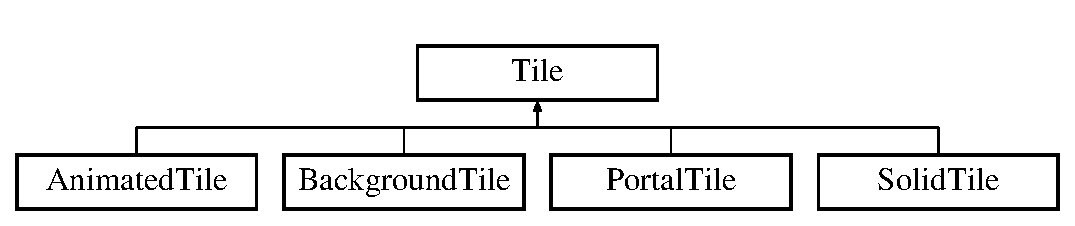
\includegraphics[height=2.000000cm]{struct_tile}
\end{center}
\end{figure}
\subsection*{Metody publiczne}
\begin{DoxyCompactItemize}
\item 
\hypertarget{struct_tile_a60143acae451458a180267fdabfd80c7}{{\bfseries Tile} (unsigned int \-\_\-x, unsigned int \-\_\-y, unsigned int \-\_\-gid)}\label{struct_tile_a60143acae451458a180267fdabfd80c7}

\end{DoxyCompactItemize}
\subsection*{Atrybuty publiczne}
\begin{DoxyCompactItemize}
\item 
\hypertarget{struct_tile_ad8ba78a01a259b052e267c754f525413}{unsigned int {\bfseries x}}\label{struct_tile_ad8ba78a01a259b052e267c754f525413}

\item 
\hypertarget{struct_tile_a33e9c4b212bbdec7eeac2f55b5b98223}{unsigned int {\bfseries y}}\label{struct_tile_a33e9c4b212bbdec7eeac2f55b5b98223}

\item 
\hypertarget{struct_tile_ac72ddfe3b77d6332c089276a0a696490}{unsigned int {\bfseries gid}}\label{struct_tile_ac72ddfe3b77d6332c089276a0a696490}

\end{DoxyCompactItemize}


\subsection{Opis szczegółowy}
struktura bazowa kafla 

Dokumentacja dla tej struktury została wygenerowana z pliku\-:\begin{DoxyCompactItemize}
\item 
Map\-System/Tiles.\-h\end{DoxyCompactItemize}

\hypertarget{class_tile_map}{\section{Dokumentacja klasy Tile\-Map}
\label{class_tile_map}\index{Tile\-Map@{Tile\-Map}}
}


Klasa renderująca mape.  




{\ttfamily \#include $<$Static\-Tiled\-Map.\-hpp$>$}

\subsection*{Metody publiczne}
\begin{DoxyCompactItemize}
\item 
void \hyperlink{class_tile_map_a6e0ee732702ceb28a6f49052f6cf1126}{set\-Item\-Manager\-Handle} (\hyperlink{class_item_manager}{Item\-Manager} $\ast$igr)
\begin{DoxyCompactList}\small\item\em Ustawia uchwyt do klasy \hyperlink{class_item_manager}{Item\-Manager}. \end{DoxyCompactList}\item 
\hypertarget{class_tile_map_a137e40e291677a1201dd96bdbd6bc6bd}{size\-\_\-t {\bfseries items\-On\-Map\-Count} () const }\label{class_tile_map_a137e40e291677a1201dd96bdbd6bc6bd}

\item 
\hypertarget{class_tile_map_a68fbe6582a01b4c565d93ddc7bde2123}{size\-\_\-t {\bfseries solid\-Tiles\-Count} () const }\label{class_tile_map_a68fbe6582a01b4c565d93ddc7bde2123}

\item 
bool \hyperlink{class_tile_map_ac084a4b6aea0e050ec4a8aeea760a515}{load\-Map} (const std\-::string name)
\begin{DoxyCompactList}\small\item\em Ładuje mape z pliku. \end{DoxyCompactList}\item 
bool \hyperlink{class_tile_map_ac5d4d6a3522663052bab1396b1116a89}{is\-Item} (sf\-::\-Vector2u, int \&\-\_\-id) const 
\begin{DoxyCompactList}\small\item\em Zwraca boola czy pod danym xy jest item. \end{DoxyCompactList}\item 
bool \hyperlink{class_tile_map_a9abb261e84ab1ce52d5f2cc6a9c43bbb}{is\-Portal} (sf\-::\-Vector2u)
\begin{DoxyCompactList}\small\item\em Zwraca bool czy xy jest portalem. \end{DoxyCompactList}\item 
bool \hyperlink{class_tile_map_aac072fd241cd09e88a256099055f7238}{pick\-Item} (sf\-::\-Vector2u)
\begin{DoxyCompactList}\small\item\em Usuwa item z mapy. \end{DoxyCompactList}\item 
bool \hyperlink{class_tile_map_ab6b915163f9462171d78d9265332c553}{drop\-Item} (const int)
\begin{DoxyCompactList}\small\item\em Dodaje item do mapy. \end{DoxyCompactList}\item 
bool \hyperlink{class_tile_map_aed48e1dfdf55facc59cbf7e7b60a80d7}{is\-Solid\-Tile} (sf\-::\-Vector2u) const 
\begin{DoxyCompactList}\small\item\em Zwraca bool czy xy jest solidną kratka. \end{DoxyCompactList}\item 
sf\-::\-Vector2f \hyperlink{class_tile_map_a53c335525a76ce71c88404a73573500e}{reload} (sf\-::\-Vector2u \&)
\begin{DoxyCompactList}\small\item\em Przeładowywuje mapke jeśli dane xy jest portalem(linkiem) \end{DoxyCompactList}\item 
int \hyperlink{class_tile_map_a3c64cb00cc8d0e38f7c24e16149fd987}{get\-G\-I\-D} (size\-\_\-t) const 
\begin{DoxyCompactList}\small\item\em Zwraca G\-I\-D itemu na podstawie I\-D. \end{DoxyCompactList}\item 
const sf\-::\-Texture \& \hyperlink{class_tile_map_ae9a8aa44841e001cad6414c517bde545}{get\-Texture} () const 
\begin{DoxyCompactList}\small\item\em Zwraca referencje do tilesetu. \end{DoxyCompactList}\item 
void \hyperlink{class_tile_map_a995c3475a7451f9b449295fbe01509f0}{refresh\-Animations} ()
\begin{DoxyCompactList}\small\item\em Odswieża animacje. \end{DoxyCompactList}\item 
void \hyperlink{class_tile_map_a28a3df759d609bc19688d48b26489718}{set\-N\-P\-C\-Manager\-Handle} (\hyperlink{class_npc_manager}{Npc\-Manager} $\ast$)
\begin{DoxyCompactList}\small\item\em Ustawia uchwyt do klasy \hyperlink{class_npc_manager}{Npc\-Manager}. \end{DoxyCompactList}\item 
\hypertarget{class_tile_map_a16fe09376fea6c92725cc3b5bb9d0a2d}{void {\bfseries print\-Solid\-Tiles} ()}\label{class_tile_map_a16fe09376fea6c92725cc3b5bb9d0a2d}

\item 
\hypertarget{class_tile_map_a105d246af258dc45a025053a0e08c860}{void {\bfseries print\-Items1} ()}\label{class_tile_map_a105d246af258dc45a025053a0e08c860}

\end{DoxyCompactItemize}


\subsection{Opis szczegółowy}
Klasa renderująca mape. 

\subsection{Dokumentacja funkcji składowych}
\hypertarget{class_tile_map_ab6b915163f9462171d78d9265332c553}{\index{Tile\-Map@{Tile\-Map}!drop\-Item@{drop\-Item}}
\index{drop\-Item@{drop\-Item}!TileMap@{Tile\-Map}}
\subsubsection[{drop\-Item}]{\setlength{\rightskip}{0pt plus 5cm}bool Tile\-Map\-::drop\-Item (
\begin{DoxyParamCaption}
\item[{const int}]{id}
\end{DoxyParamCaption}
)}}\label{class_tile_map_ab6b915163f9462171d78d9265332c553}


Dodaje item do mapy. 

Wyszukuje item o danym id (id są unikalne) w itemach gracza (Klasie \hyperlink{class_item_manager}{Item\-Manager}) i usuwa ją z vectora w tej klasie, a następnie dodaje do itemków na mapie 
\begin{DoxyParams}{Parametry}
{\em id} & id itemu \\
\hline
\end{DoxyParams}
\begin{DoxyReturn}{Zwraca}
Jeśli istnieje item o takim id true w przeciwnym wypadku false 
\end{DoxyReturn}
\hypertarget{class_tile_map_a3c64cb00cc8d0e38f7c24e16149fd987}{\index{Tile\-Map@{Tile\-Map}!get\-G\-I\-D@{get\-G\-I\-D}}
\index{get\-G\-I\-D@{get\-G\-I\-D}!TileMap@{Tile\-Map}}
\subsubsection[{get\-G\-I\-D}]{\setlength{\rightskip}{0pt plus 5cm}int Tile\-Map\-::get\-G\-I\-D (
\begin{DoxyParamCaption}
\item[{size\-\_\-t}]{id}
\end{DoxyParamCaption}
) const}}\label{class_tile_map_a3c64cb00cc8d0e38f7c24e16149fd987}


Zwraca G\-I\-D itemu na podstawie I\-D. 

Wyszukuje w vectorze itemów na mapie itemu o danym id i zwraca jego G\-I\-D 
\begin{DoxyParams}{Parametry}
{\em id} & id przedmiotu \\
\hline
\end{DoxyParams}
\begin{DoxyReturn}{Zwraca}
G\-I\-D przedmiotu jeśli istnieje item o takim id na mapie, w przeciwnym wypadku -\/1 
\end{DoxyReturn}
\hypertarget{class_tile_map_ae9a8aa44841e001cad6414c517bde545}{\index{Tile\-Map@{Tile\-Map}!get\-Texture@{get\-Texture}}
\index{get\-Texture@{get\-Texture}!TileMap@{Tile\-Map}}
\subsubsection[{get\-Texture}]{\setlength{\rightskip}{0pt plus 5cm}const sf\-::\-Texture \& Tile\-Map\-::get\-Texture (
\begin{DoxyParamCaption}
{}
\end{DoxyParamCaption}
) const}}\label{class_tile_map_ae9a8aa44841e001cad6414c517bde545}


Zwraca referencje do tilesetu. 

\begin{DoxyReturn}{Zwraca}
sf\-::\-Texture\& 
\end{DoxyReturn}
\hypertarget{class_tile_map_ac5d4d6a3522663052bab1396b1116a89}{\index{Tile\-Map@{Tile\-Map}!is\-Item@{is\-Item}}
\index{is\-Item@{is\-Item}!TileMap@{Tile\-Map}}
\subsubsection[{is\-Item}]{\setlength{\rightskip}{0pt plus 5cm}bool Tile\-Map\-::is\-Item (
\begin{DoxyParamCaption}
\item[{sf\-::\-Vector2u}]{vct, }
\item[{int \&}]{\-\_\-id}
\end{DoxyParamCaption}
) const}}\label{class_tile_map_ac5d4d6a3522663052bab1396b1116a89}


Zwraca boola czy pod danym xy jest item. 

Zwraca boola czy pod danym xy jest item, i jeśli tak ustawia przez referencje jego id, jeśli nie to przez referencje zosanie ustawione -\/1 
\begin{DoxyParams}{Parametry}
{\em vct} & współrzędne \-\_\-id referencja do inta \\
\hline
\end{DoxyParams}
\begin{DoxyReturn}{Zwraca}
true i id w referencji jeśli xy to item false i -\/1 w referencji jeśli xy nie jest itemem 
\end{DoxyReturn}
\hypertarget{class_tile_map_a9abb261e84ab1ce52d5f2cc6a9c43bbb}{\index{Tile\-Map@{Tile\-Map}!is\-Portal@{is\-Portal}}
\index{is\-Portal@{is\-Portal}!TileMap@{Tile\-Map}}
\subsubsection[{is\-Portal}]{\setlength{\rightskip}{0pt plus 5cm}bool Tile\-Map\-::is\-Portal (
\begin{DoxyParamCaption}
\item[{sf\-::\-Vector2u}]{vct}
\end{DoxyParamCaption}
)}}\label{class_tile_map_a9abb261e84ab1ce52d5f2cc6a9c43bbb}


Zwraca bool czy xy jest portalem. 

Zwraca bool czy xy jest portalem ( linkiem do innej mapy ) 
\begin{DoxyParams}{Parametry}
{\em vct} & współrzędne \\
\hline
\end{DoxyParams}
\begin{DoxyReturn}{Zwraca}
true jeśli portal, w przeciwnym wypadku false 
\end{DoxyReturn}
\hypertarget{class_tile_map_aed48e1dfdf55facc59cbf7e7b60a80d7}{\index{Tile\-Map@{Tile\-Map}!is\-Solid\-Tile@{is\-Solid\-Tile}}
\index{is\-Solid\-Tile@{is\-Solid\-Tile}!TileMap@{Tile\-Map}}
\subsubsection[{is\-Solid\-Tile}]{\setlength{\rightskip}{0pt plus 5cm}bool Tile\-Map\-::is\-Solid\-Tile (
\begin{DoxyParamCaption}
\item[{sf\-::\-Vector2u}]{vct}
\end{DoxyParamCaption}
) const}}\label{class_tile_map_aed48e1dfdf55facc59cbf7e7b60a80d7}


Zwraca bool czy xy jest solidną kratka. 

Zwraca bool czy xy jest solidna kratka (taka na którą nie można wejść) 
\begin{DoxyParams}{Parametry}
{\em vct} & współrzędne \\
\hline
\end{DoxyParams}
\begin{DoxyReturn}{Zwraca}
Jeśli xy solidne true, w przeciwnym wypadku false 
\end{DoxyReturn}
\hypertarget{class_tile_map_ac084a4b6aea0e050ec4a8aeea760a515}{\index{Tile\-Map@{Tile\-Map}!load\-Map@{load\-Map}}
\index{load\-Map@{load\-Map}!TileMap@{Tile\-Map}}
\subsubsection[{load\-Map}]{\setlength{\rightskip}{0pt plus 5cm}bool Tile\-Map\-::load\-Map (
\begin{DoxyParamCaption}
\item[{const std\-::string}]{name}
\end{DoxyParamCaption}
)}}\label{class_tile_map_ac084a4b6aea0e050ec4a8aeea760a515}


Ładuje mape z pliku. 

Niepowodzenia zapisuje do pliku z logiem 
\begin{DoxyParams}{Parametry}
{\em name} & nazwa mapy do załadowania \\
\hline
\end{DoxyParams}
\begin{DoxyReturn}{Zwraca}
Powodzenie operacji 
\end{DoxyReturn}
\hypertarget{class_tile_map_aac072fd241cd09e88a256099055f7238}{\index{Tile\-Map@{Tile\-Map}!pick\-Item@{pick\-Item}}
\index{pick\-Item@{pick\-Item}!TileMap@{Tile\-Map}}
\subsubsection[{pick\-Item}]{\setlength{\rightskip}{0pt plus 5cm}bool Tile\-Map\-::pick\-Item (
\begin{DoxyParamCaption}
\item[{sf\-::\-Vector2u}]{xy}
\end{DoxyParamCaption}
)}}\label{class_tile_map_aac072fd241cd09e88a256099055f7238}


Usuwa item z mapy. 

Wyszukuje w wektorze itemów na mapie itema o danym xy i usuwa go, dodaje item o danym id do Item\-Managera i ustawia mu flage picked w klasie \hyperlink{class_item_manager}{Item\-Manager} (oznacza to że item został podniesiony z mapy raz i przy kolejnym załadowaniu mapy już nie zostanie wyrenderowany) docelowo flagi picked będą zapisywane w save (ale to jest T\-O\-D\-O) 
\begin{DoxyParams}{Parametry}
{\em xy} & wektor z pozycją gracza \\
\hline
\end{DoxyParams}
\begin{DoxyReturn}{Zwraca}
Jeśli item podniesiony true, jeśli pod współrzędnymi nie ma itema to false 
\end{DoxyReturn}
\hypertarget{class_tile_map_a995c3475a7451f9b449295fbe01509f0}{\index{Tile\-Map@{Tile\-Map}!refresh\-Animations@{refresh\-Animations}}
\index{refresh\-Animations@{refresh\-Animations}!TileMap@{Tile\-Map}}
\subsubsection[{refresh\-Animations}]{\setlength{\rightskip}{0pt plus 5cm}void Tile\-Map\-::refresh\-Animations (
\begin{DoxyParamCaption}
{}
\end{DoxyParamCaption}
)}}\label{class_tile_map_a995c3475a7451f9b449295fbe01509f0}


Odswieża animacje. 

Resetuje zegar i zmienia klatki animacji na mapie \hypertarget{class_tile_map_a53c335525a76ce71c88404a73573500e}{\index{Tile\-Map@{Tile\-Map}!reload@{reload}}
\index{reload@{reload}!TileMap@{Tile\-Map}}
\subsubsection[{reload}]{\setlength{\rightskip}{0pt plus 5cm}sf\-::\-Vector2f Tile\-Map\-::reload (
\begin{DoxyParamCaption}
\item[{sf\-::\-Vector2u \&}]{vct}
\end{DoxyParamCaption}
)}}\label{class_tile_map_a53c335525a76ce71c88404a73573500e}


Przeładowywuje mapke jeśli dane xy jest portalem(linkiem) 

Przeładowywuje mapke (czyści tablice vertexów, oraz itemy na mapie) ustawia współrzędne gracza i wywołuje metode \hyperlink{class_tile_map_ac084a4b6aea0e050ec4a8aeea760a515}{load\-Map()} 
\begin{DoxyParams}{Parametry}
{\em vct} & Współrzędne \\
\hline
\end{DoxyParams}
\begin{DoxyReturn}{Zwraca}
Nowe współrzędne w których ma pojawić sie gracz lub wektor(0,0) jeśli błąd 
\end{DoxyReturn}
\hypertarget{class_tile_map_a6e0ee732702ceb28a6f49052f6cf1126}{\index{Tile\-Map@{Tile\-Map}!set\-Item\-Manager\-Handle@{set\-Item\-Manager\-Handle}}
\index{set\-Item\-Manager\-Handle@{set\-Item\-Manager\-Handle}!TileMap@{Tile\-Map}}
\subsubsection[{set\-Item\-Manager\-Handle}]{\setlength{\rightskip}{0pt plus 5cm}void Tile\-Map\-::set\-Item\-Manager\-Handle (
\begin{DoxyParamCaption}
\item[{{\bf Item\-Manager} $\ast$}]{igr}
\end{DoxyParamCaption}
)}}\label{class_tile_map_a6e0ee732702ceb28a6f49052f6cf1126}


Ustawia uchwyt do klasy \hyperlink{class_item_manager}{Item\-Manager}. 

Klasa mapy potrzebuje informacji o itemach i dlatego potrzebny jest tu uchwyt \hypertarget{class_tile_map_a28a3df759d609bc19688d48b26489718}{\index{Tile\-Map@{Tile\-Map}!set\-N\-P\-C\-Manager\-Handle@{set\-N\-P\-C\-Manager\-Handle}}
\index{set\-N\-P\-C\-Manager\-Handle@{set\-N\-P\-C\-Manager\-Handle}!TileMap@{Tile\-Map}}
\subsubsection[{set\-N\-P\-C\-Manager\-Handle}]{\setlength{\rightskip}{0pt plus 5cm}void Tile\-Map\-::set\-N\-P\-C\-Manager\-Handle (
\begin{DoxyParamCaption}
\item[{{\bf Npc\-Manager} $\ast$}]{\-\_\-hnd}
\end{DoxyParamCaption}
)}}\label{class_tile_map_a28a3df759d609bc19688d48b26489718}


Ustawia uchwyt do klasy \hyperlink{class_npc_manager}{Npc\-Manager}. 

Ustawia uchwyt do klasy \hyperlink{class_npc_manager}{Npc\-Manager} 

Dokumentacja dla tej klasy została wygenerowana z plików\-:\begin{DoxyCompactItemize}
\item 
Map\-System/Static\-Tiled\-Map.\-hpp\item 
Map\-System/Static\-Tiled\-Map.\-cpp\end{DoxyCompactItemize}

\printindex
\end{document}
